% Overrides original definition
\def\rmhtmet{\mbox{$\mathcal{R}$}\xspace}

%%____________________________________________________________________________||
\section{Background estimation for QCD multijet events \label{sec:qcd}}
\subsection{QCD control with the \bdphi variable}

One of the major challenges for searches of new physics in the jets +
\met final state is the control of background events from QCD multijet
production. The difficulties in the determination of precise estimates
for this background stem from the large cross sections expected in the
high-energy, high-luminosity hadron collider environment at the LHC,
which are further compounded by the lack of precise theoretical
predictions for the cross sections and kinematic properties of
multijet events. Hence, without special consideration and treatment,
significant uncertainties on large background expectations can
overwhelm any potential sensitivity to new physics signatures.

With regards to QCD multijet production, the approach of this search
is to favour the suppression of the multijet background to a
negligible level over the goal of high efficiency for any given signal
model. A conservative uncertainty on a negligible contribution is
preferred over a procedure that attempts to accurately estimate a
non-negligible contribution from multijet events. The level of
contamination should be sufficiently small (\ie sub-percent level)
such that the associated uncertainty, even if large, will be
sub-dominant with respect to the uncertainties on the remaining SM
backgrounds with genuine \met such as \wj, \znunu, and \ttbar,
henceforth labelled as non-multijet processes.

Any contamination from QCD multijet events is controlled primarily
through the \alphat and \bdphi variables. The \alphat variable is able
to distinguish with high efficiency the sources of ``fake'' \met, such
as jet energy mismeasurement, from those with ``genuine'' \met, such
as neutrinos. The \bdphi variable is also very efficient at
identifying jets that suffer under-measurements, as well as
over-measurements, in (otherwise balanced) multijet events. The
variable is also particularly suited to identifying multijet events
that exhibit significant \met due to the production of neutrinos
(collinear with a jet axis) in semileptonic heavy-flavour decays. Both
variables are individually capable of reducing the yields from
multijet events by several orders of magnitude, and combined provide
an extremely robust method to reject multijet events.

In Fig.~\ref{fig:bDPhi_nominal} a comparison of the abilities of the \bdphi variable to 
control the QCD multijet background with 
a similar jet-\mht angular variable \dphimhtj, the minimum azimuthal separation between the \mht-vector and the leading four
jets, is presented. The \bdphi variable exhibits a distribution that
is more sharply peaked for the QCD multijet background 
at low values and faster falling than \dphimhtj,  \dphimhtj for QCD conversely has a broader 
distribution with a larger leakage for a comparable azimuthal
selection. This demonstrates the ability of \bdphi to provide a better
control of the QCD background while retaining acceptance of events with genuine \mht,
in this case represented by the V+jets, \ttbar and other residual SM
backgrounds with genuine \met. 

This is
further demonstrated in Fig.~\ref{fig:bDPhi_roc}, where the efficiency
of retaining processes with genuine \mht is plotted against the
background efficiency for a series of \bdphi, \dphimhtj and
\dphimhtjall cuts, where \dphimhtjall considers all jets rather than
just the leading four. The
points with a cut of $0.5$ are highlighted as stars on the plot. The
general analysis strategy involves reducing the QCD multijet
background to a negligible level while maximising signal acceptance. These plots demonstrate that this is
most achievable with a cut on \bdphi. For the same threshold
requirement of $0.5$ on each variable, the \bdphi variable provides an
efficiency for multijet events that is approximately three orders of
magnitude lower than for \dphimhtj at the cost of approximately a factor $3$
reduction in signal efficiency. The threshold on \bdphi required to give
an approximately equivalent suppression of QCD achieved with the
\dphimhtj
variable is larger than 1.5, at the cost of a loss of a factor $5$ in
signal acceptance w.r.t. \bdphi. This also holds true in the extreme
case of a high jet multiplicity signal model. Additionally, despite
performing similarly to \bdphi for separating the non-multijet from
multijet backgrounds, the \dphimhtjall variable performs worse for a
high jet multiplicity signal model than \bdphi.

Additionally the \bdphi variable displays robustness in the 
presence of severe event mismeasurement. A mismeasurement is simulated by artificially lowering 
the \pt of the jet that minimises the azimuthal separation variable to 41 \GeV and the event 
variables recomputed. Due to the removal of the probe jet from the computation of \bdphi, the 
distribution of angular separation Fig.~\ref{fig:shifted_bDPhi_dist} is 
remains unchanged under severe mismeasurement. The \dphimhtj variable is
 sensitive to such mismeasurement as both \mht and the rank of the 
leading four jets are affected, resulting in a broader distribution with
increased leakage Fig.~\ref{fig:shifted_DPhiMht_dist}.

\begin{figure}[!h]
 \centering
 \subfigure[\bdphi distribution.\label{fig:bDPhi_dist}]{
 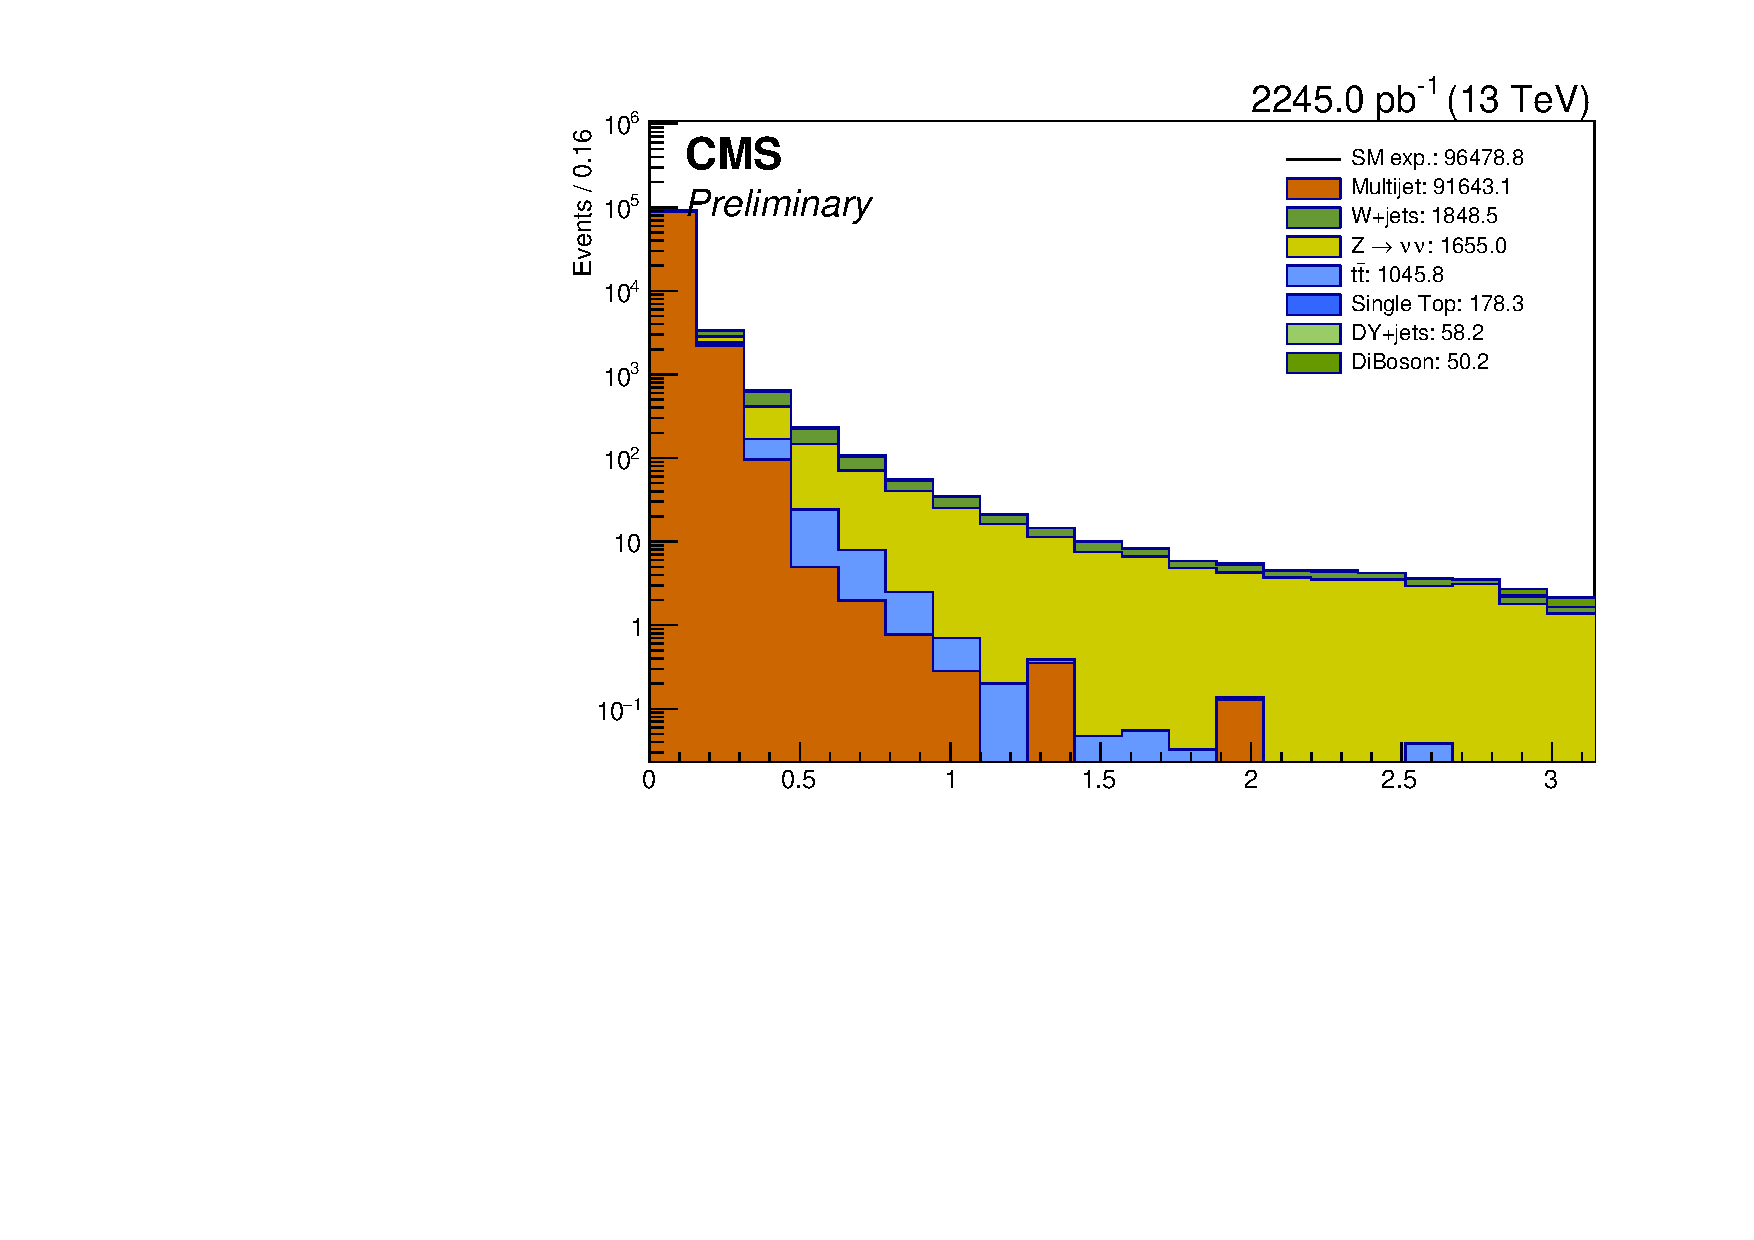
\includegraphics[width=0.5\textwidth]{figures/qcd/biasedDPhi_all_800}
 }
 \subfigure[\dphimhtj distribution.\label{fig:DPhiMht_dist}]{
 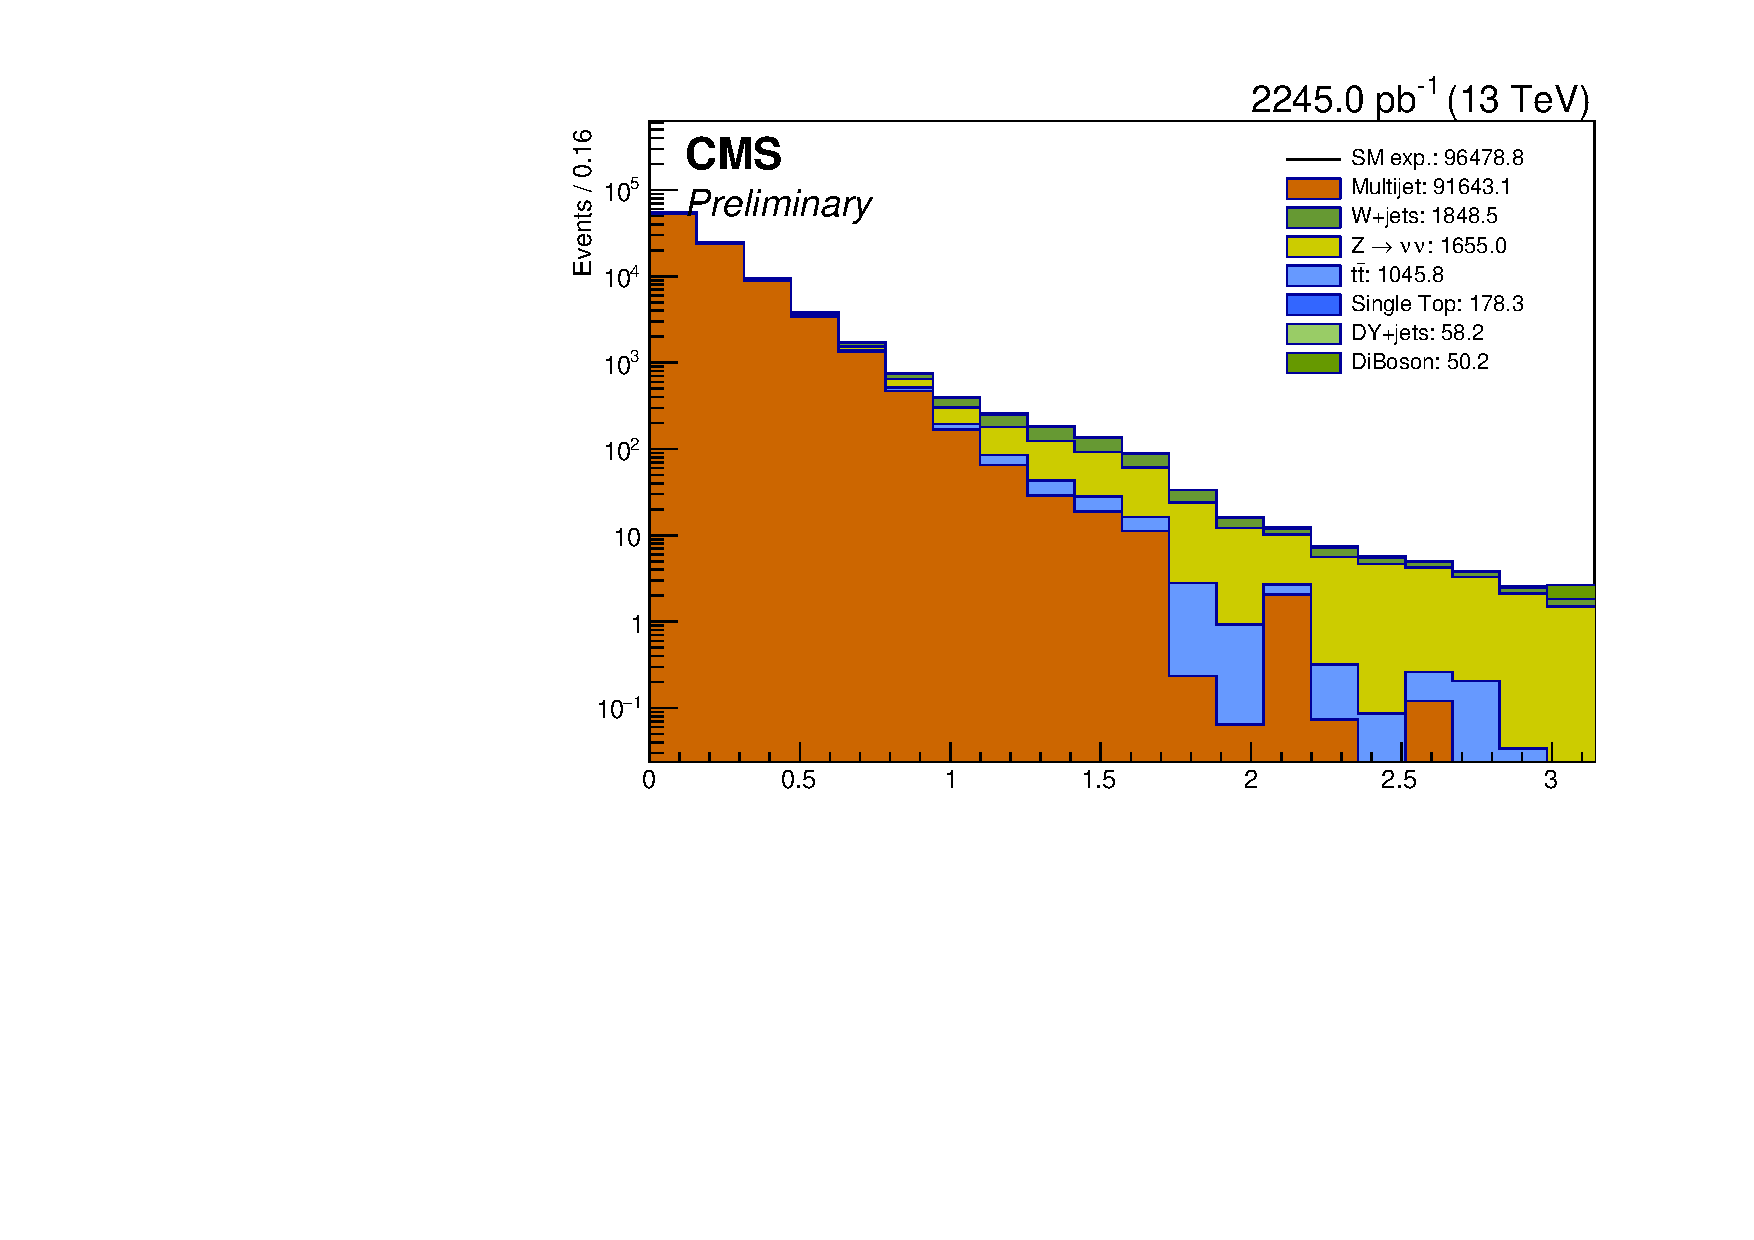
\includegraphics[width=0.5\textwidth]{figures/qcd/minDeltaPhiMht_all_800}
 } \\
 \caption{\bdphi and \dphimhtj distributions of MC simulation of the
 dominant analysis backgrounds
 after analysis selections for \scalht $> 800$ \GeV. }
 \label{fig:bDPhi_nominal}
\end{figure}

\begin{figure}[!h]
 \centering
 \subfigure[Acceptance of SM backgrounds with genuine \met vs QCD
 acceptance]{
 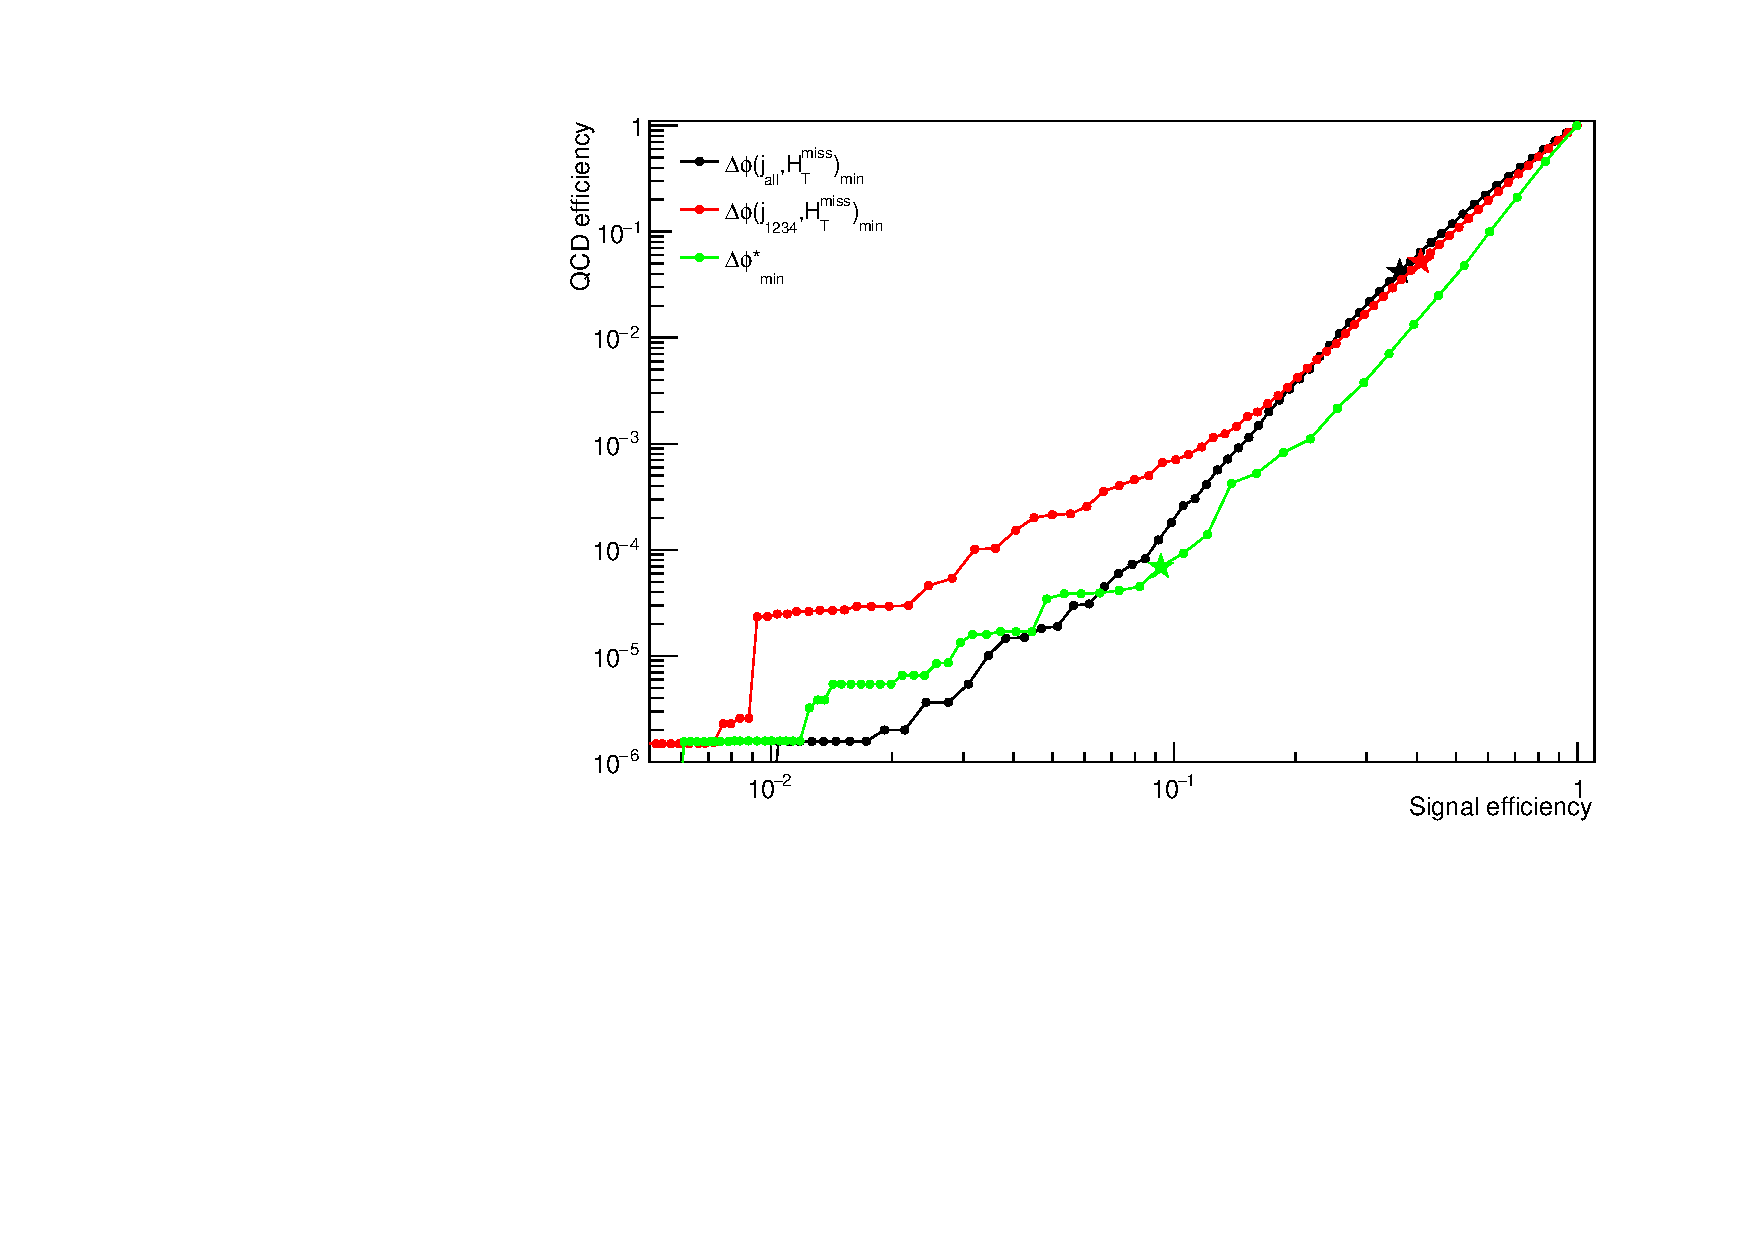
\includegraphics[width=0.5\textwidth]{figures/qcd/rateEffEwkQCD}
 }~
 \subfigure[High jet multiplicity signal acceptance vs QCD acceptance]{
 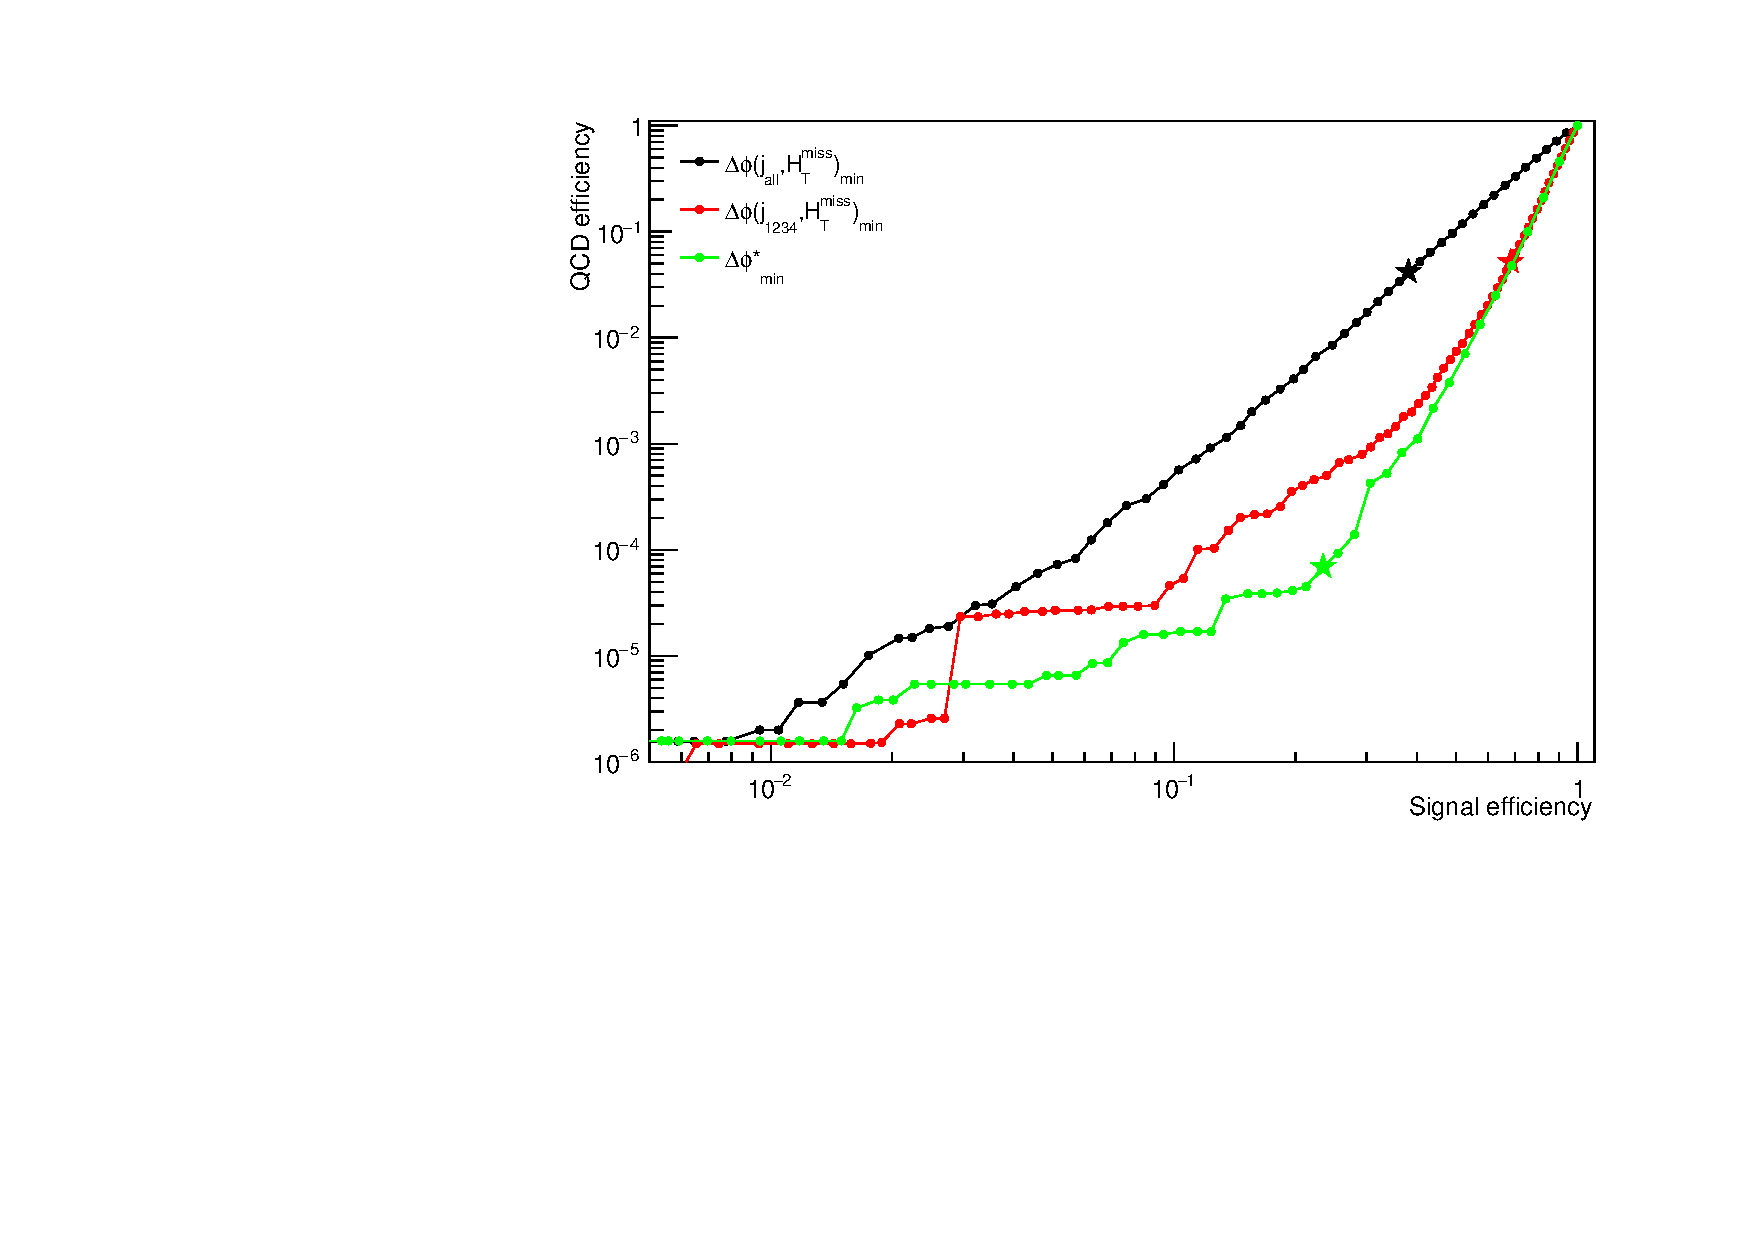
\includegraphics[width=0.5\textwidth]{figures/qcd/rateEffSignalQCD}
 } \\
 \caption{\bdphi, \dphimhtj and \dphimhtjall efficiency for simulation of processes with genuine
 \met vs QCD multijet background efficiency. The stars correspond to
 efficiencies with a cut of $0.5$ on each variable. A generic case of
 non-multijet process efficiency is considered in (a). In (b) we
 consider an uncompressed T1tttt model. This is the case in which \bdphi is
 expected to have the lowest efficiency due to the very high jet
 multiplicity of the model.}
 \label{fig:bDPhi_roc}
\end{figure}

\begin{figure}[!h]
 \centering
 \subfigure[QCD \bdphi distribution with mismeasurement.\label{fig:shifted_bDPhi_dist}]{
 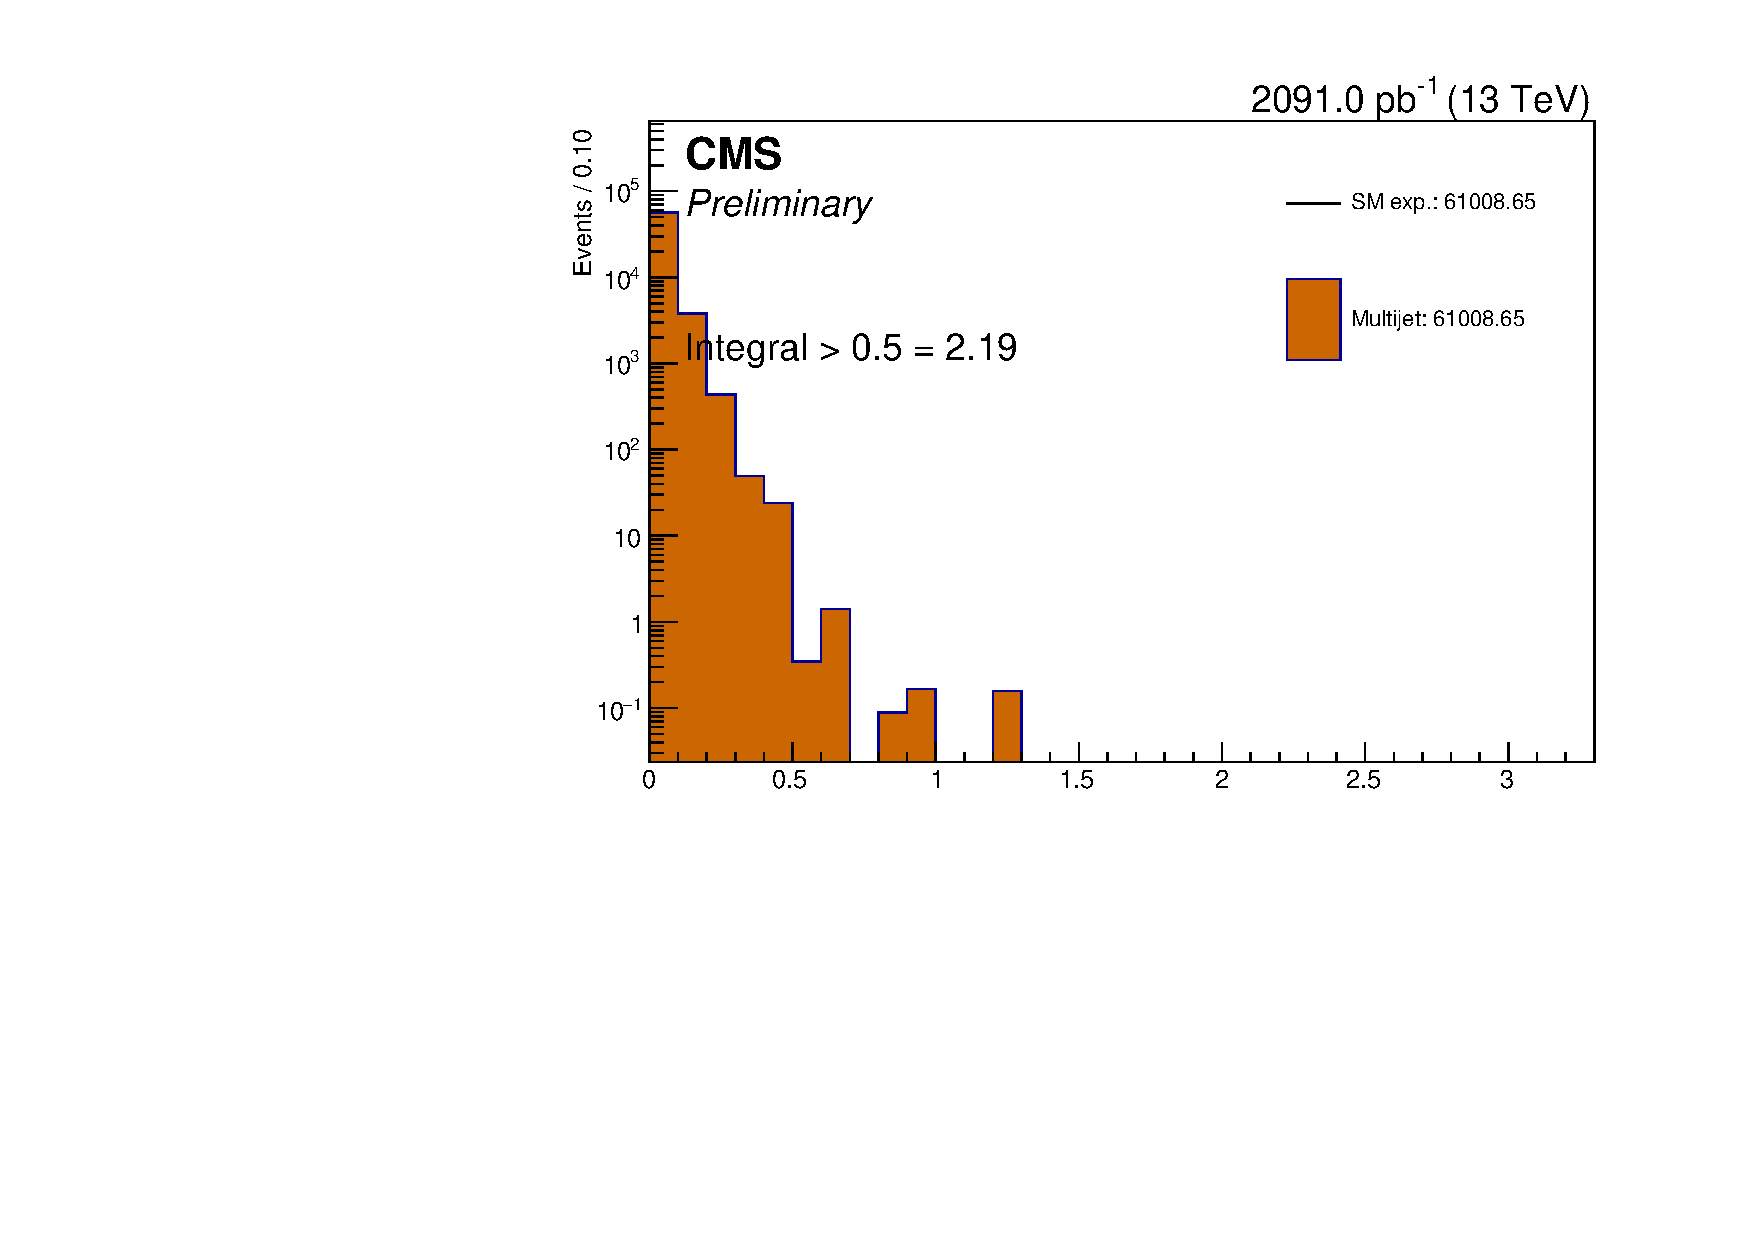
\includegraphics[width=0.5\textwidth]{figures/qcd/v6/bDPhi/shiftedMinBDPhi_all_800}
 }
 \subfigure[QCD \dphimhtj distribution with mismeasurement.\label{fig:shifted_DPhiMht_dist}]{
 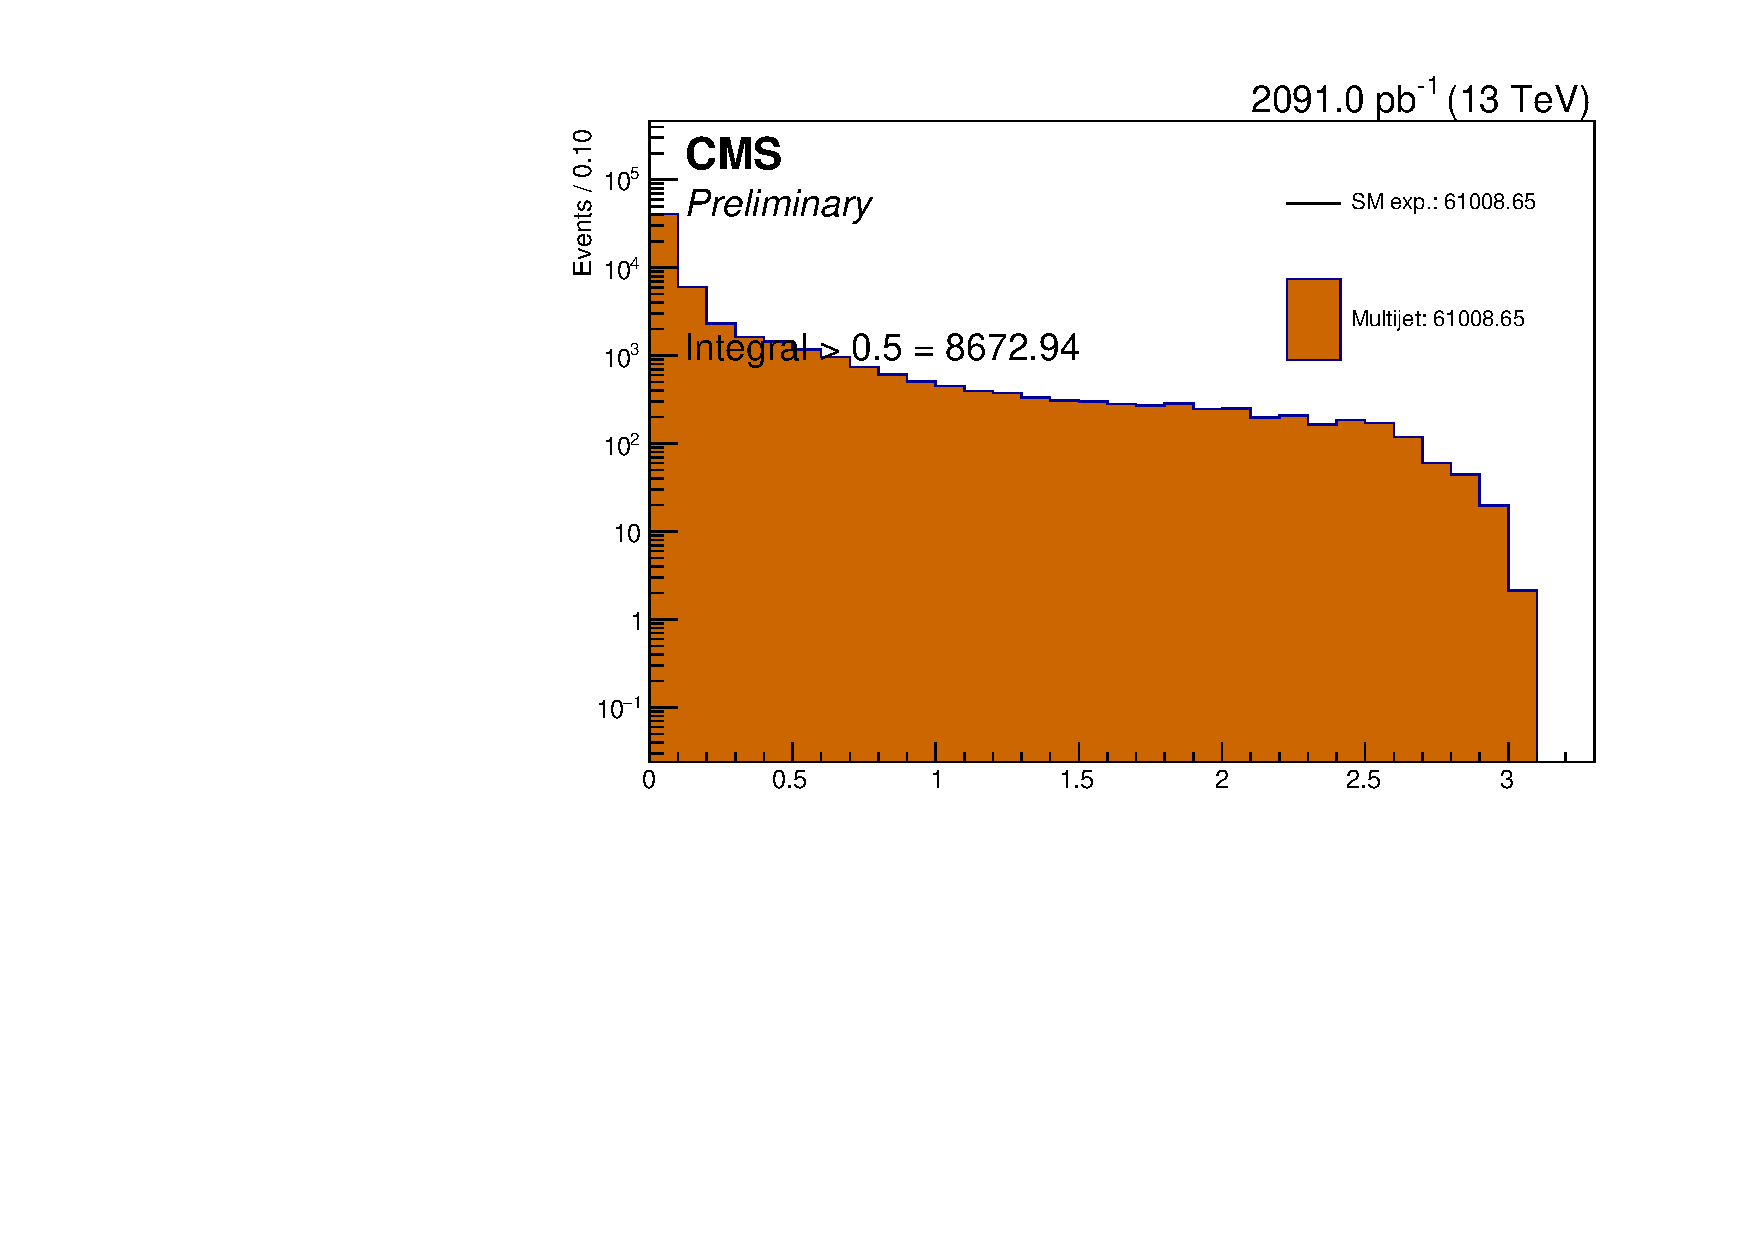
\includegraphics[width=0.5\textwidth]{figures/qcd/v6/bDPhi/shiftedMinDeltaPhiMht_all_800}
 } \\
 \caption{\bdphi and \dphimhtj distributions of QCD multijet simulation
 after analysis selections for \scalht $> 800$ \GeV in the case of
 severe mismeasurement. The
 total number of events that pass a $\Delta\phi > 0.5$ selection of the
 respective quantity are indicated. (N.B. these plots were made with
 an older iteration of the analysis and have not been fully updated,
 although their conclusions remain true)}
 \label{fig:bDPhi_mismeasured}
\end{figure}

\subsection{The method and results}
\label{sec:qcdMethod}

%FIXME Could reword this to remove the references to Run 1?
In Run~1, the \alphat and \bdphi thresholds that reduced
multijet contamination to the required level were determined by a
dedicated data-driven method, which relied on multijet-enriched
sidebands in the variables \alphat, \bdphi, and \mhtmet. The \mhtmet
variable, discussed in Sec.~\ref{sec:selection}, is used to filter QCD
multijet events that contain soft jets below threshold contributing
significantly to \mht. The method relied on extrapolating the
exponential modelling of the number of multijet events passing and
failing a requirement on the variable \mhtmet, \ie the pass/fail ratio
\rmhtmet, as a function of \alphat for a given signal region bin
(defined in terms of \njet, \nb, and \scalht). In essence, the
approach employed was an ABCD method that accounted for the
correlation between the variables \rmhtmet and \alphat, followed
by an additional requirement on \bdphi determined and validated in a
data control sideband.

For this search, we employ a simpler approach that relies on the
determination of the ratio \rmhtmet per (\njet,\scalht) bin from
simulation. The ratio is determined following the application of the
\alphat and \bdphi requirements, which in the former case are
\scalht-dependent. For the region $\scalht > 800\gev$, the requirement
$\mht > 130\gev$ is made in place of any on \alphat. No \alphat nor
\mht requirements are imposed for events in the monojet
category.\footnote{For events in the monojet bin, an implicit
  requirement of $\mht > 200\gev$ is indeed made given that $\mht =
  \scalht$ for monojet events. No \alphat calculation can be made
  given the absence of a second jet.} The requirements on \alphat,
\mht, and \bdphi as a function of \scalht are summarised in
Sec.~\ref{sec:selection}. 

Each ratio, \rmhtmet, is used as a
multiplier on the predicted QCD counts per (\njet,\scalht) bin in a
\mhtmet data sideband. 
These data counts are collected with the
\verb!HLT_HTxxx_AlphaT0pyy!  and \verb!HLT_HT800! signal triggers
described in Sec.~\ref{sec:triggers}. 

In order to obtain an estimate of the number
of QCD multijet events in the sideband, $\mathcal{Q}$, a maximum likelihood fit analagous to that
described in Sec.~\ref{sec:likelihood} is performed. In this
fit, the
electroweak backgrounds are determined with the method described in
Sec.~\ref{sec:ewk-method} with single muon, double muon
and single photon control regions that have the same selection as the control regions
described in Sec.~\ref{sec:selection}, apart from an inverted \mhtmet
cut. All relevant systematic uncertainties are taken into account,
including the shape uncertainties described in
Sec.~\ref{sec:mc-variations} and the data driven uncertainties
uncertainties described in Sec.~\ref{sec:closure-tests}. 
After the contribution of the electroweak backgrounds is
estimated, the
remaining data counts are attributed to QCD. In this prediction, all
counts and predictions are inclusive in \nb. The
product of these predicted QCD counts and the ratio, $\mathcal{Q} \times
\rmhtmet$, provides an estimate of the level of QCD multijet events in
each (\njet,\scalht) bin of the signal region. The estimate is
currently made inclusively with respect to the \nb\ and \mht for each
(\njet,\scalht) bin. 

\begin{figure}[!h]
  \centering
  \subfigure[Simulated QCD events in signal region.\label{fig:qcd_pass}]{
    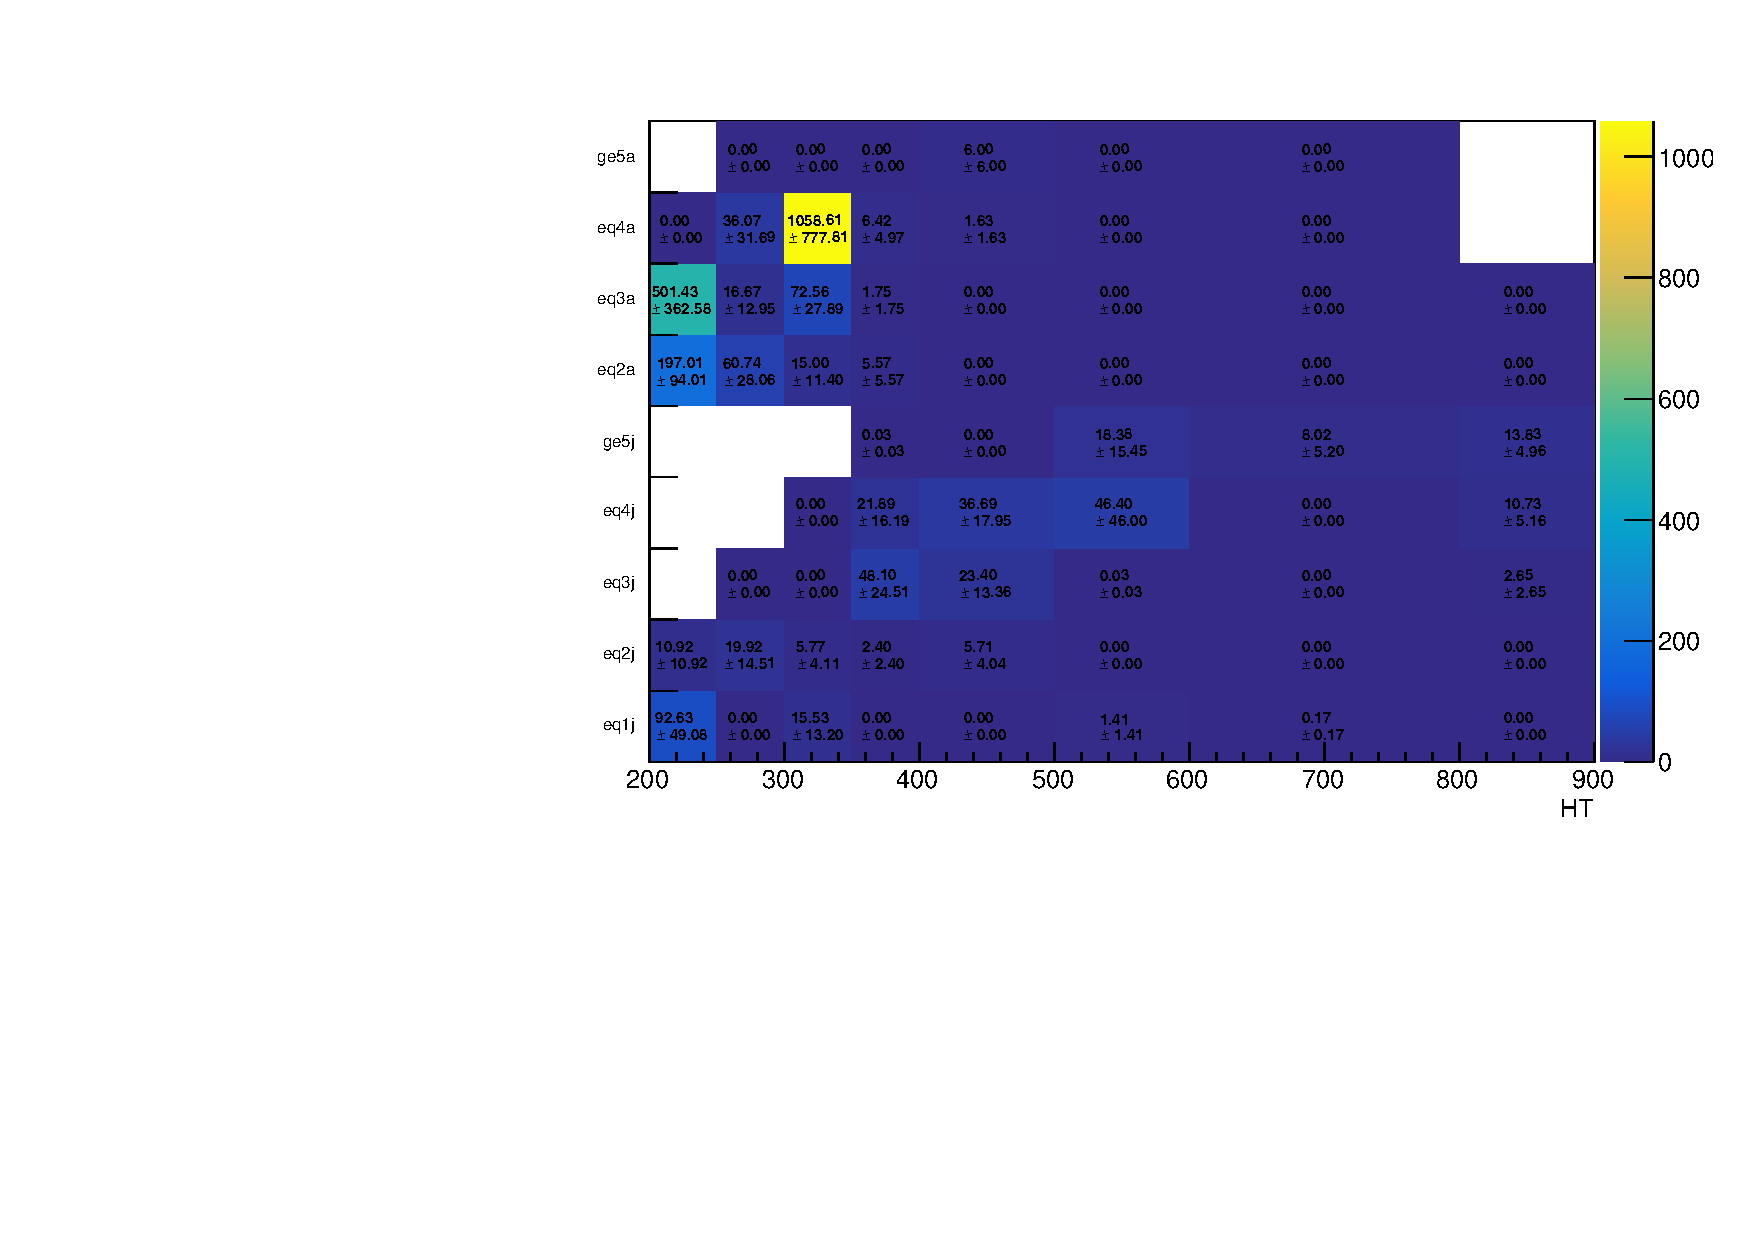
\includegraphics[width=0.5\textwidth]{figures/qcd/plots/signalQCD_MC}
  } 
  \subfigure[Simulated QCD events in \mhtmet sideband.\label{fig:qcd_fail}]{
    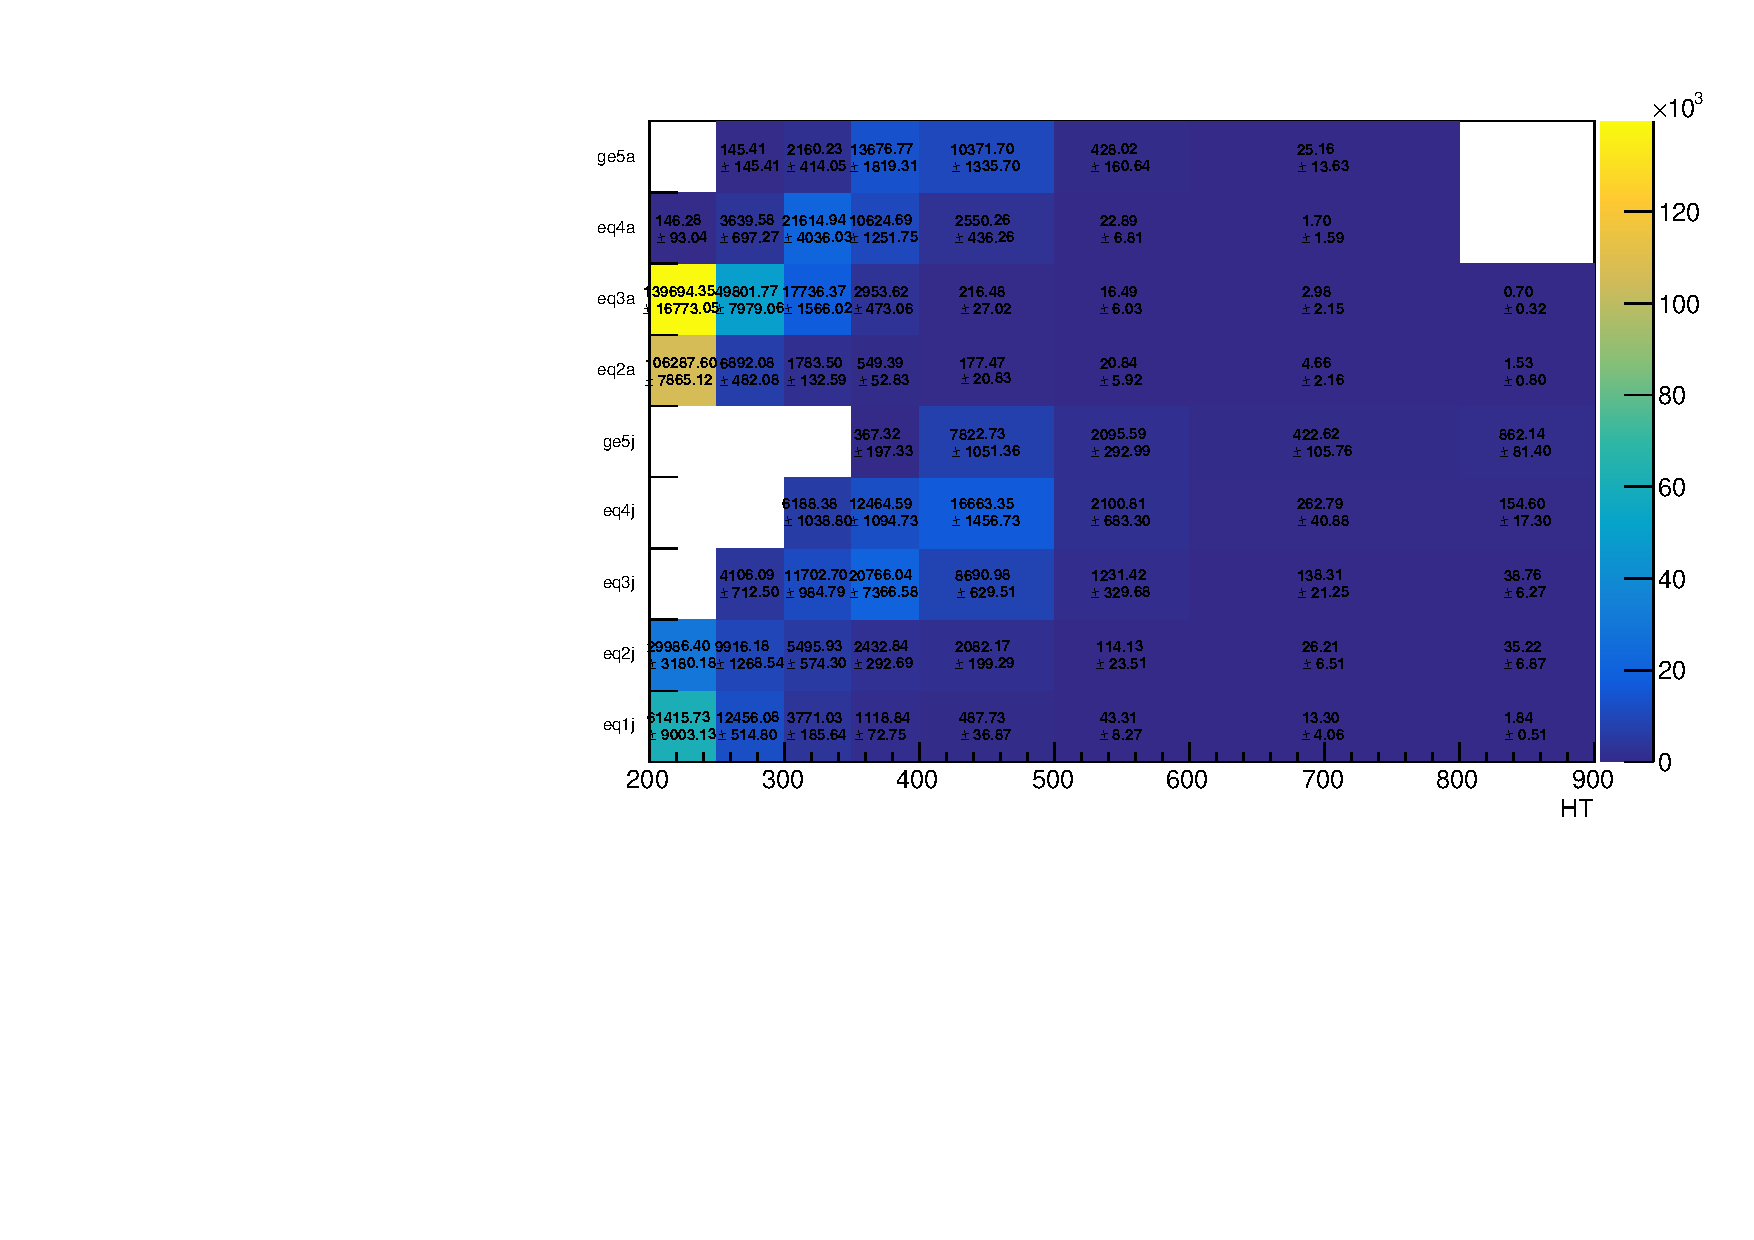
\includegraphics[width=0.5\textwidth]{figures/qcd/plots/qcdSbQCD_MC}
  } \\
  \subfigure[Ratio \rmhtmet for simulated QCD events.\label{fig:qcd_ratio}]{
    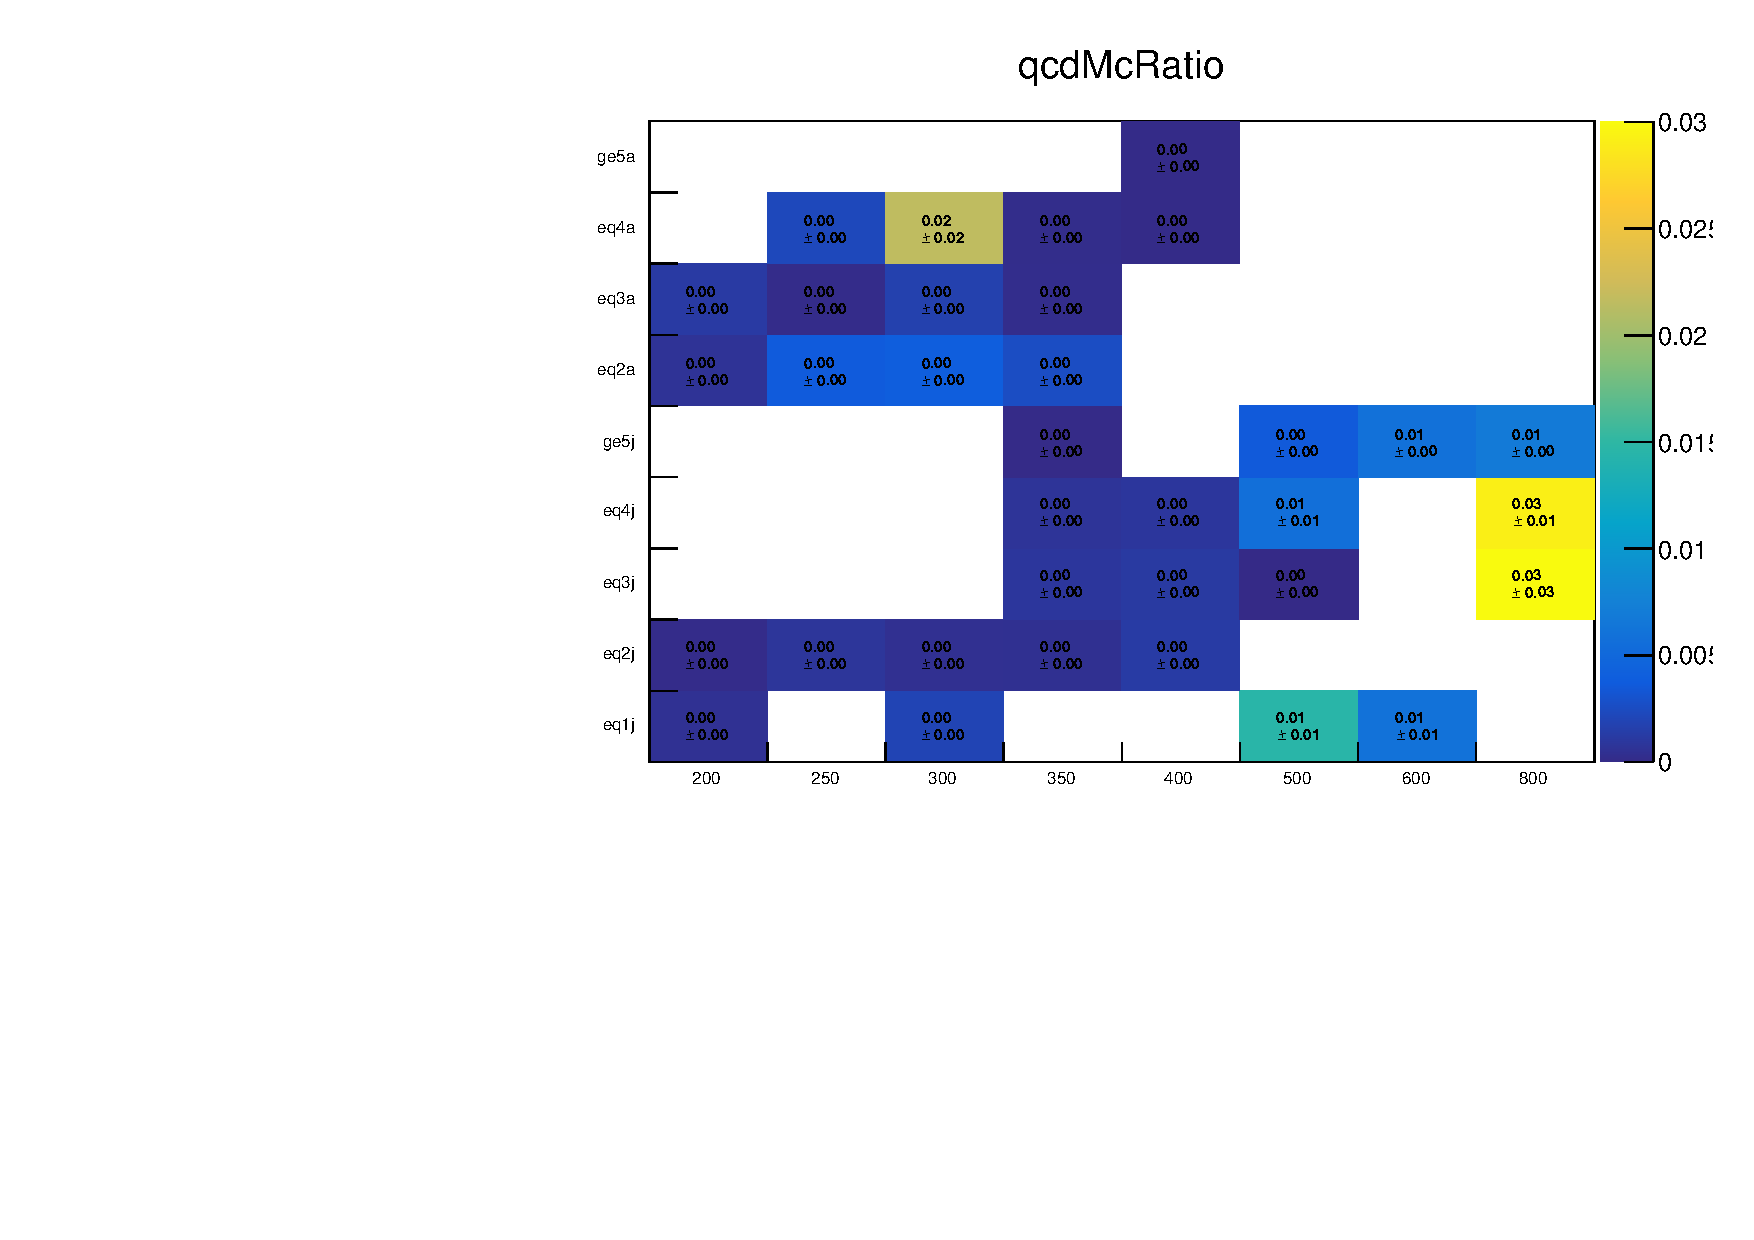
\includegraphics[width=0.5\textwidth]{figures/qcd/plots/signalQcdDivSbQcd_MC}
  } 
  \subfigure[Simulated EWK events in \mhtmet sideband.\label{fig:ewk_fail}]{
    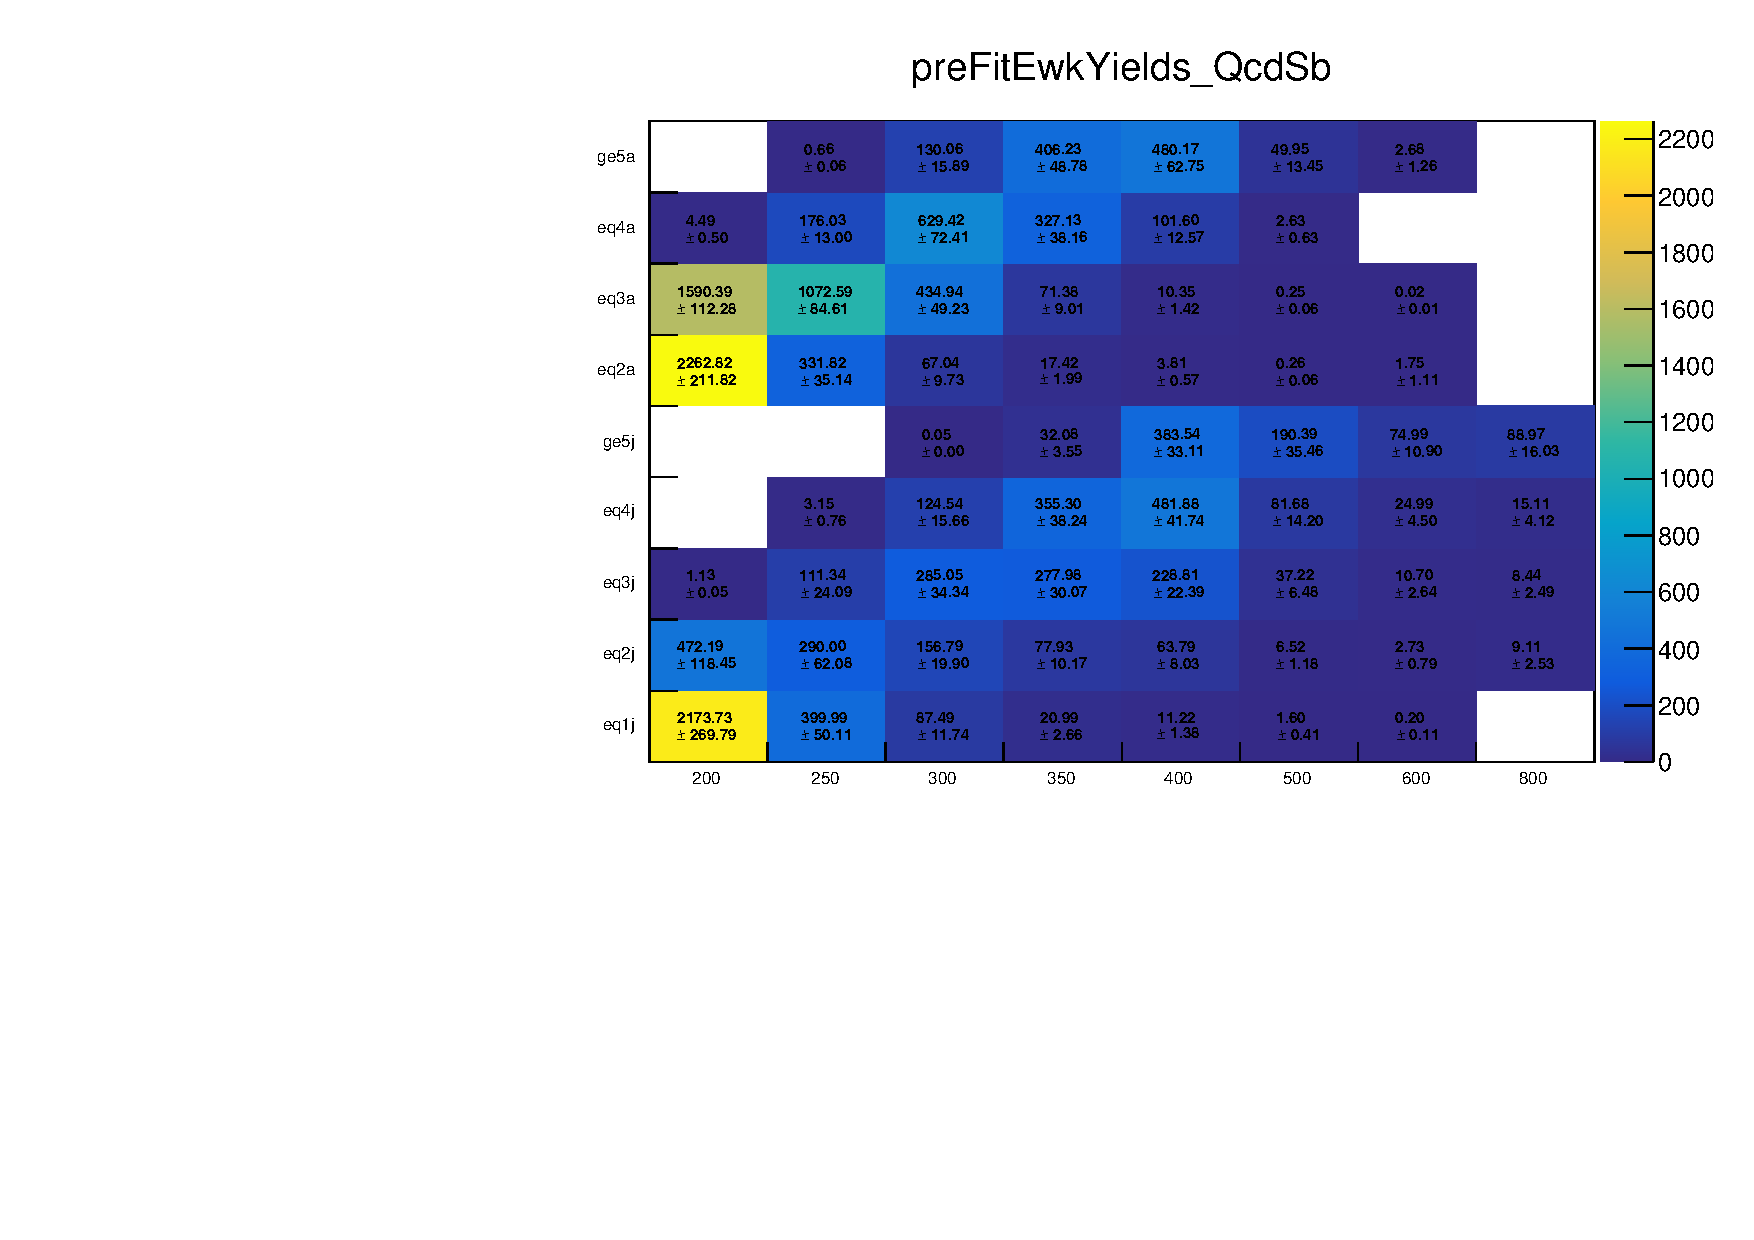
\includegraphics[width=0.5\textwidth]{figures/qcd/plots/qcdSbEwk_MC}
   %    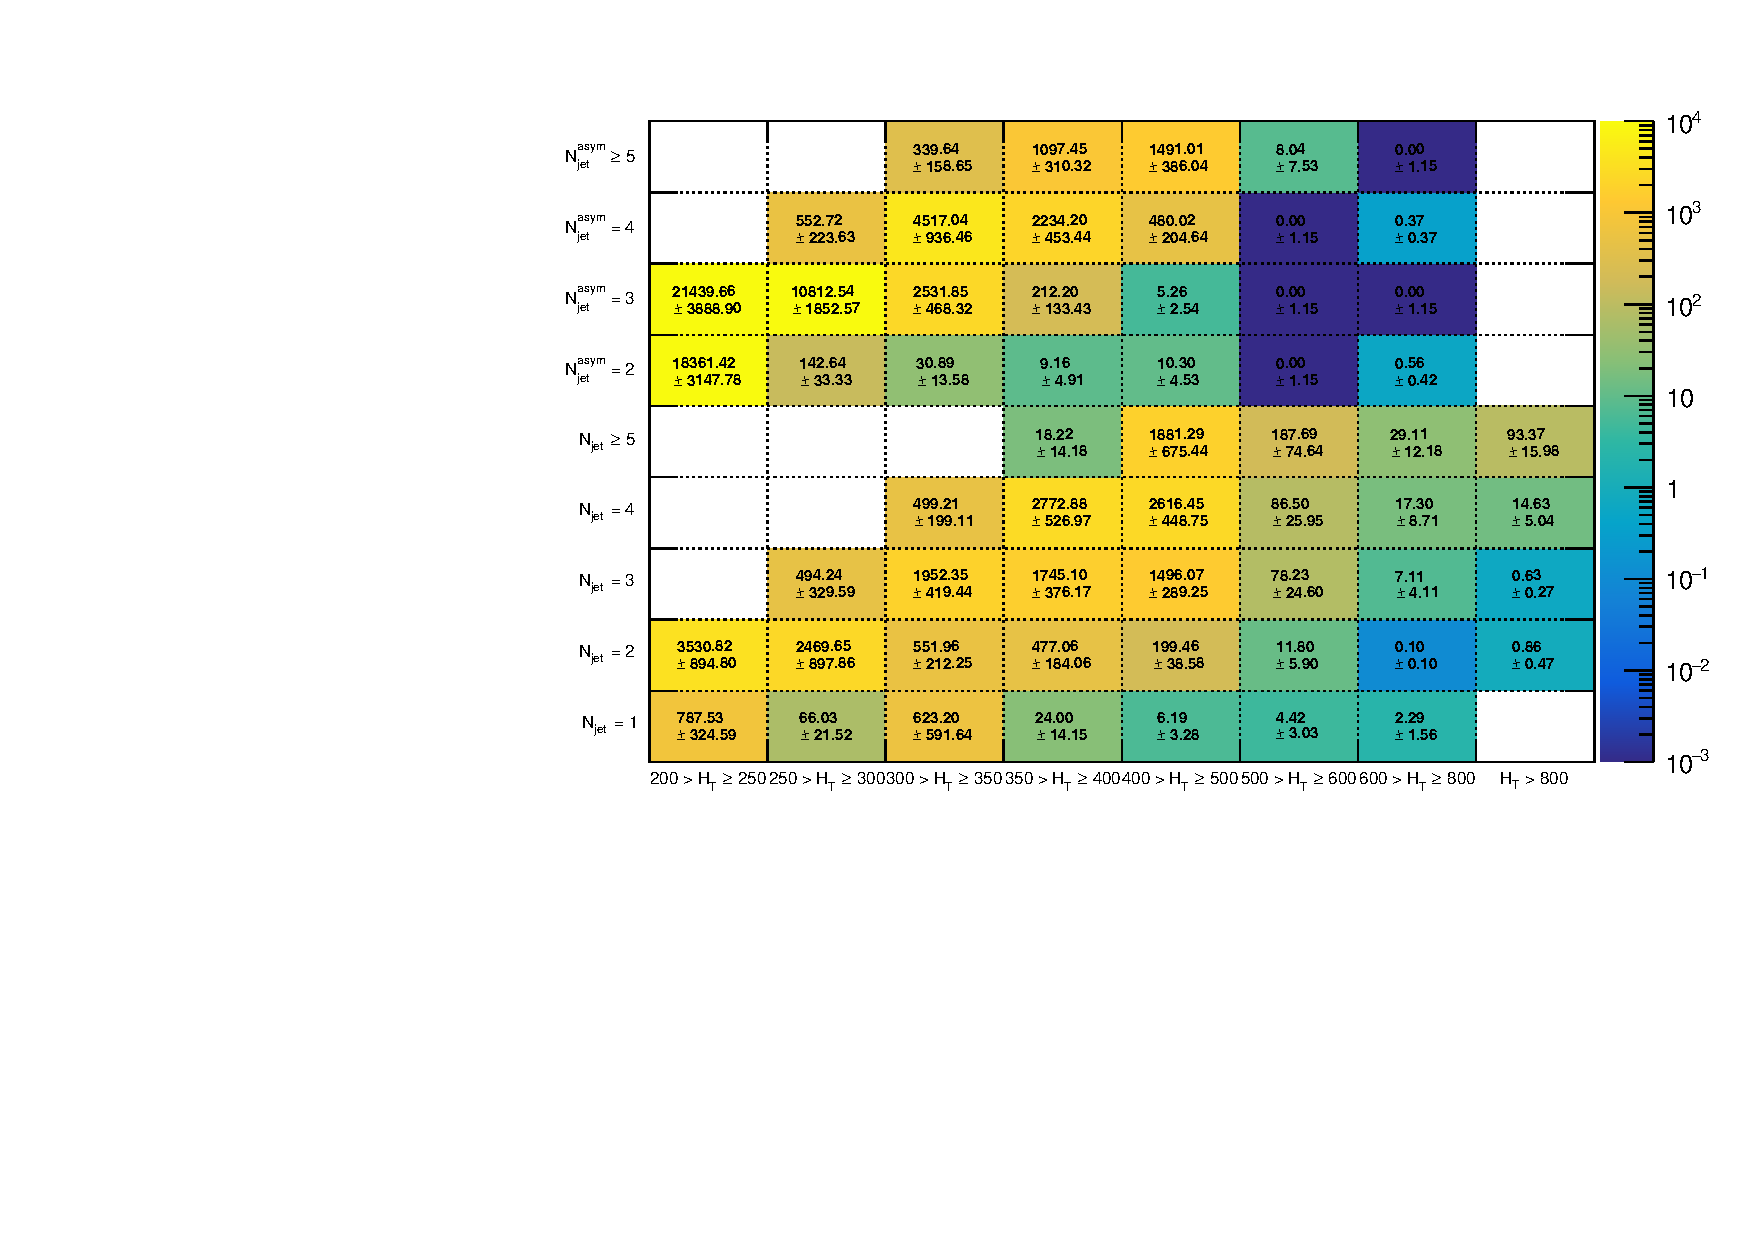
\includegraphics[width=0.5\textwidth]{figures/qcd/v6/Ewk/SigTrig_FailMoM_NJet_vs_HT_bDPhigt0p5_Log}
  } \\
  \caption{Expected number of QCD multijet events determined from
    simulation, binned according to \njet and \scalht, that (a) satisfy
    and (b) fail the requirement $\mhtmet < 1.25$. Also shown in (c)
    is the ratio \rmhtmet for QCD multijets, again determined from
    simulation. Finally, (d) shows the expected number of EWK events
    (V+jets and \ttbar, plus other residual non-multijet backgrounds)
    that fail the $\mhtmet < 1.25$ requirement, again determined from
    simulation and binned according to \njet and \scalht.}
  \label{fig:qcd_plots}
\end{figure}

The number of counts from multijet events satisfying and failing the
requirement $\mhtmet < 1.25$, \ie the pass/fail ratio \rmhtmet, are summarised in Fig.~\ref{fig:qcd_pass},
\ref{fig:qcd_fail}, and \ref{fig:qcd_ratio}. Figure~\ref{fig:ewk_fail}
shows the expected counts from non-multijet backgrounds in the \mhtmet
sideband, as determined from simulation.

\begin{figure}[!h]
  \centering
  \subfigure[Binned data counts in \mhtmet sideband.\label{fig:data_fail}]{
    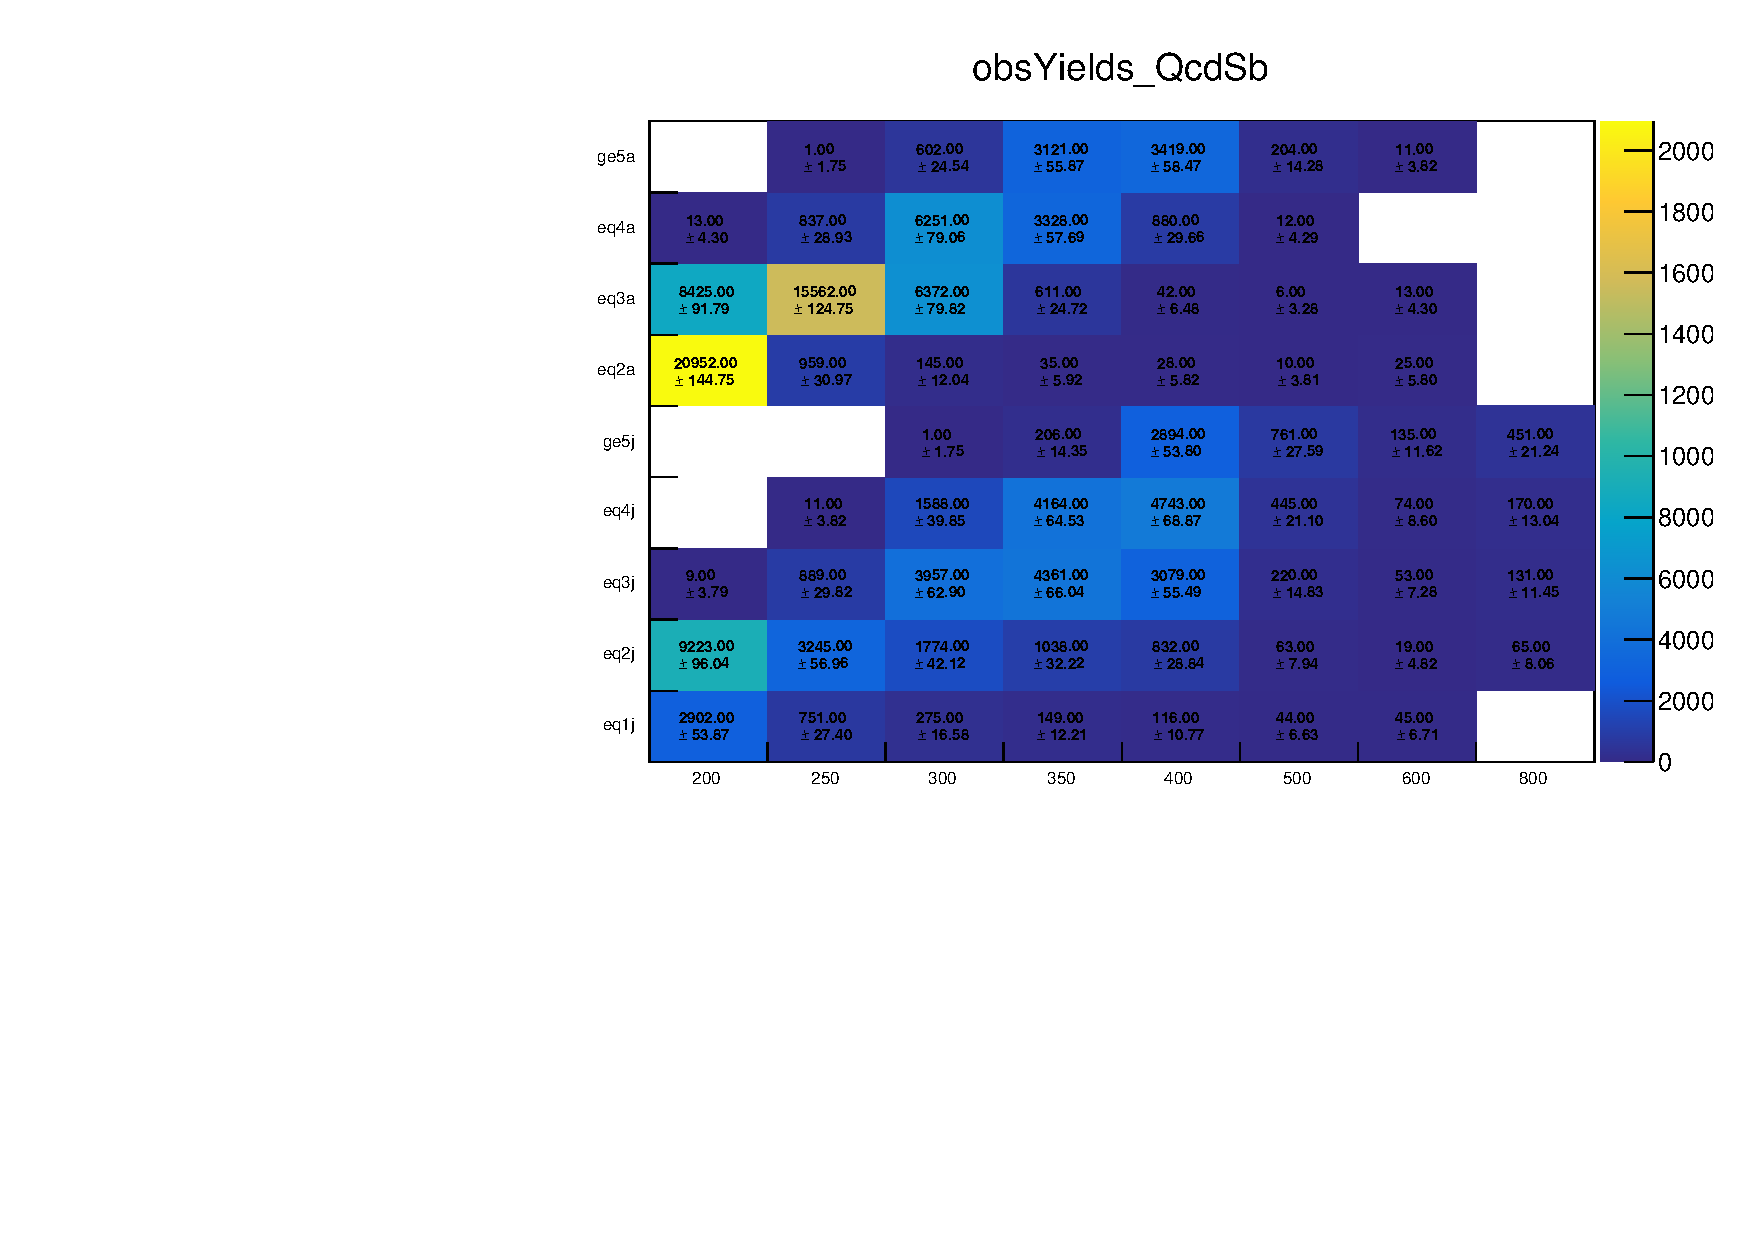
\includegraphics[width=0.5\textwidth]{figures/qcd/plots/obsYields_QcdSb}
  } 
  \subfigure[Predicted QCD counts in \mhtmet sideband.\label{fig:data_corr}]{
    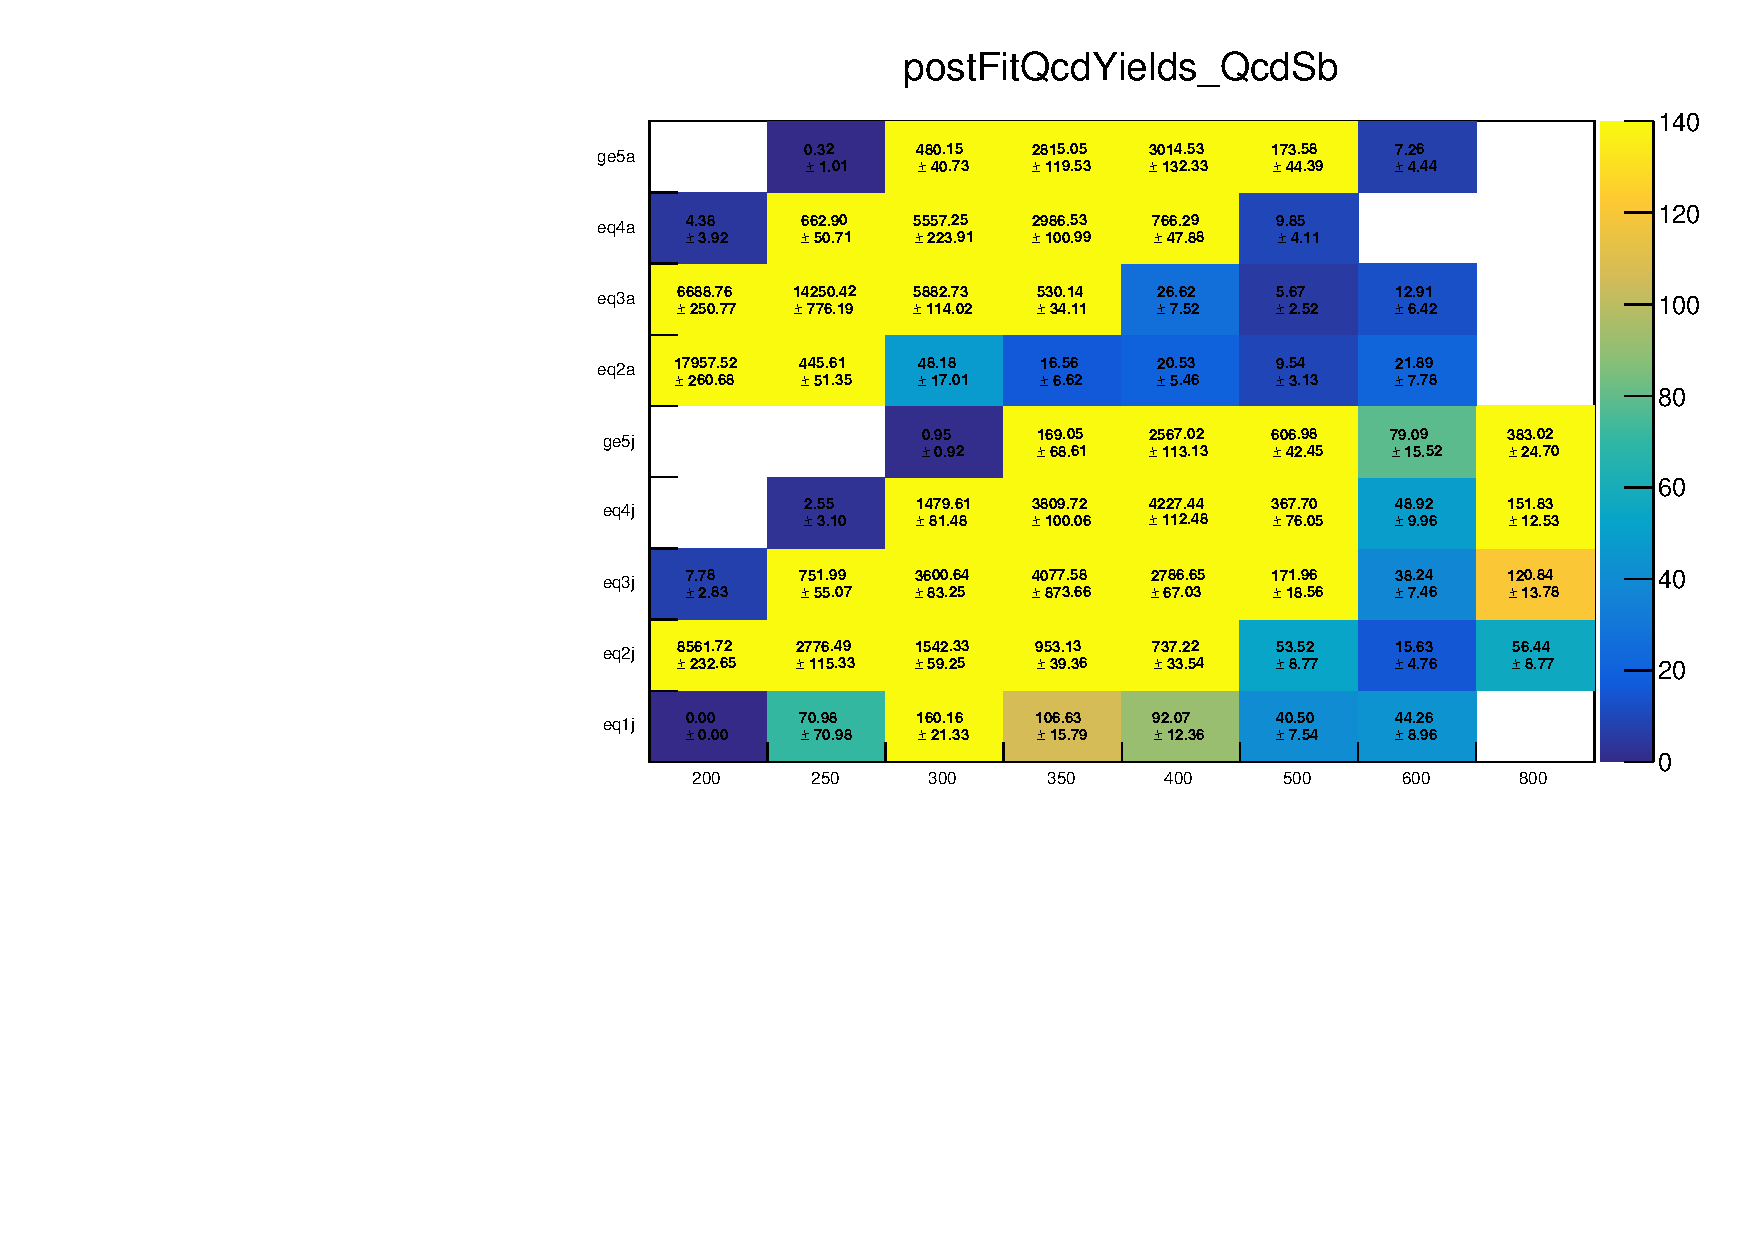
\includegraphics[width=0.5\textwidth]{figures/qcd/plots/postFitQcdYields_QcdSb}
  } \\
  \subfigure[QCD multijet predictions in the signal region.\label{fig:qcd_pred}]{
    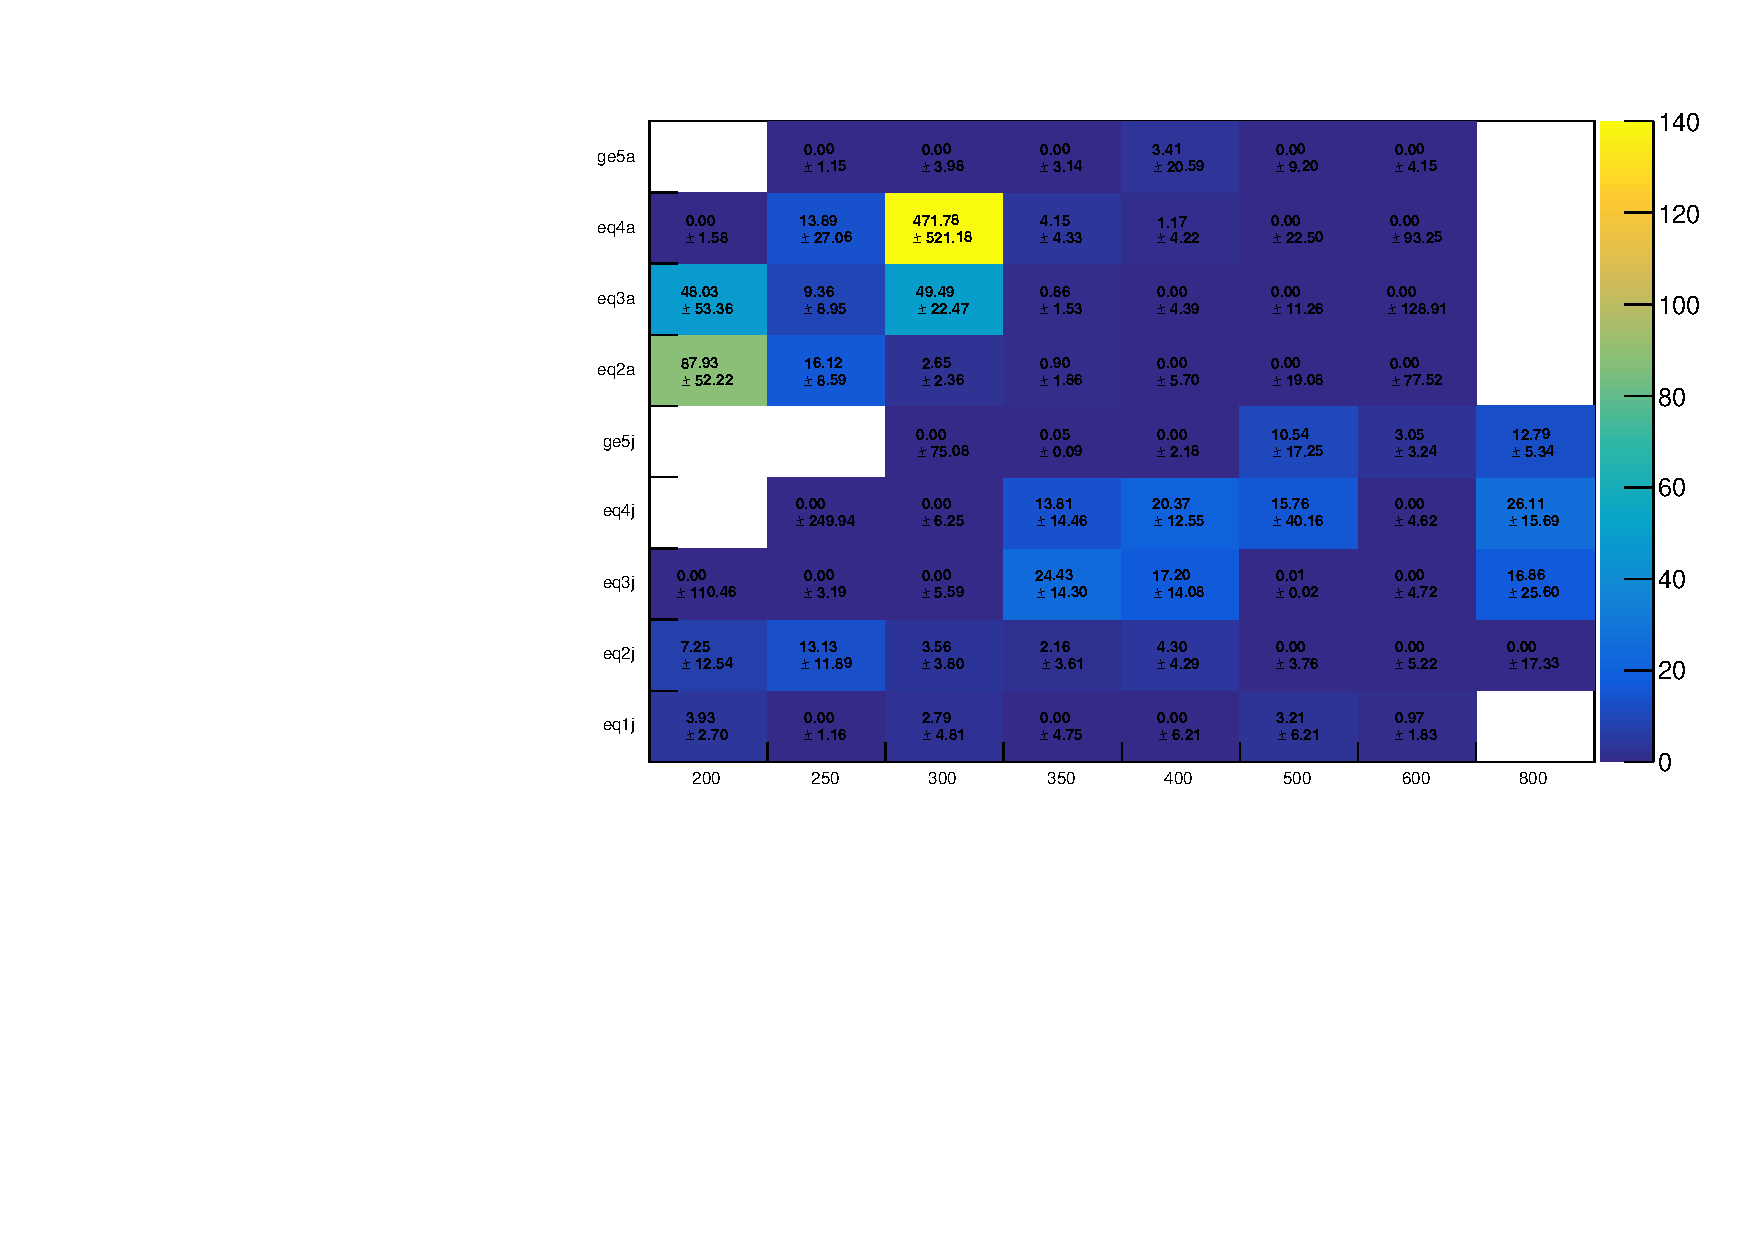
\includegraphics[width=0.5\textwidth]{figures/qcd/plots/predictedQcdYields_Signal}
  } 
  \subfigure[Ratio of predicted multijet and non-multijet yields.\label{fig:qcd_ewk_ratio}]{
    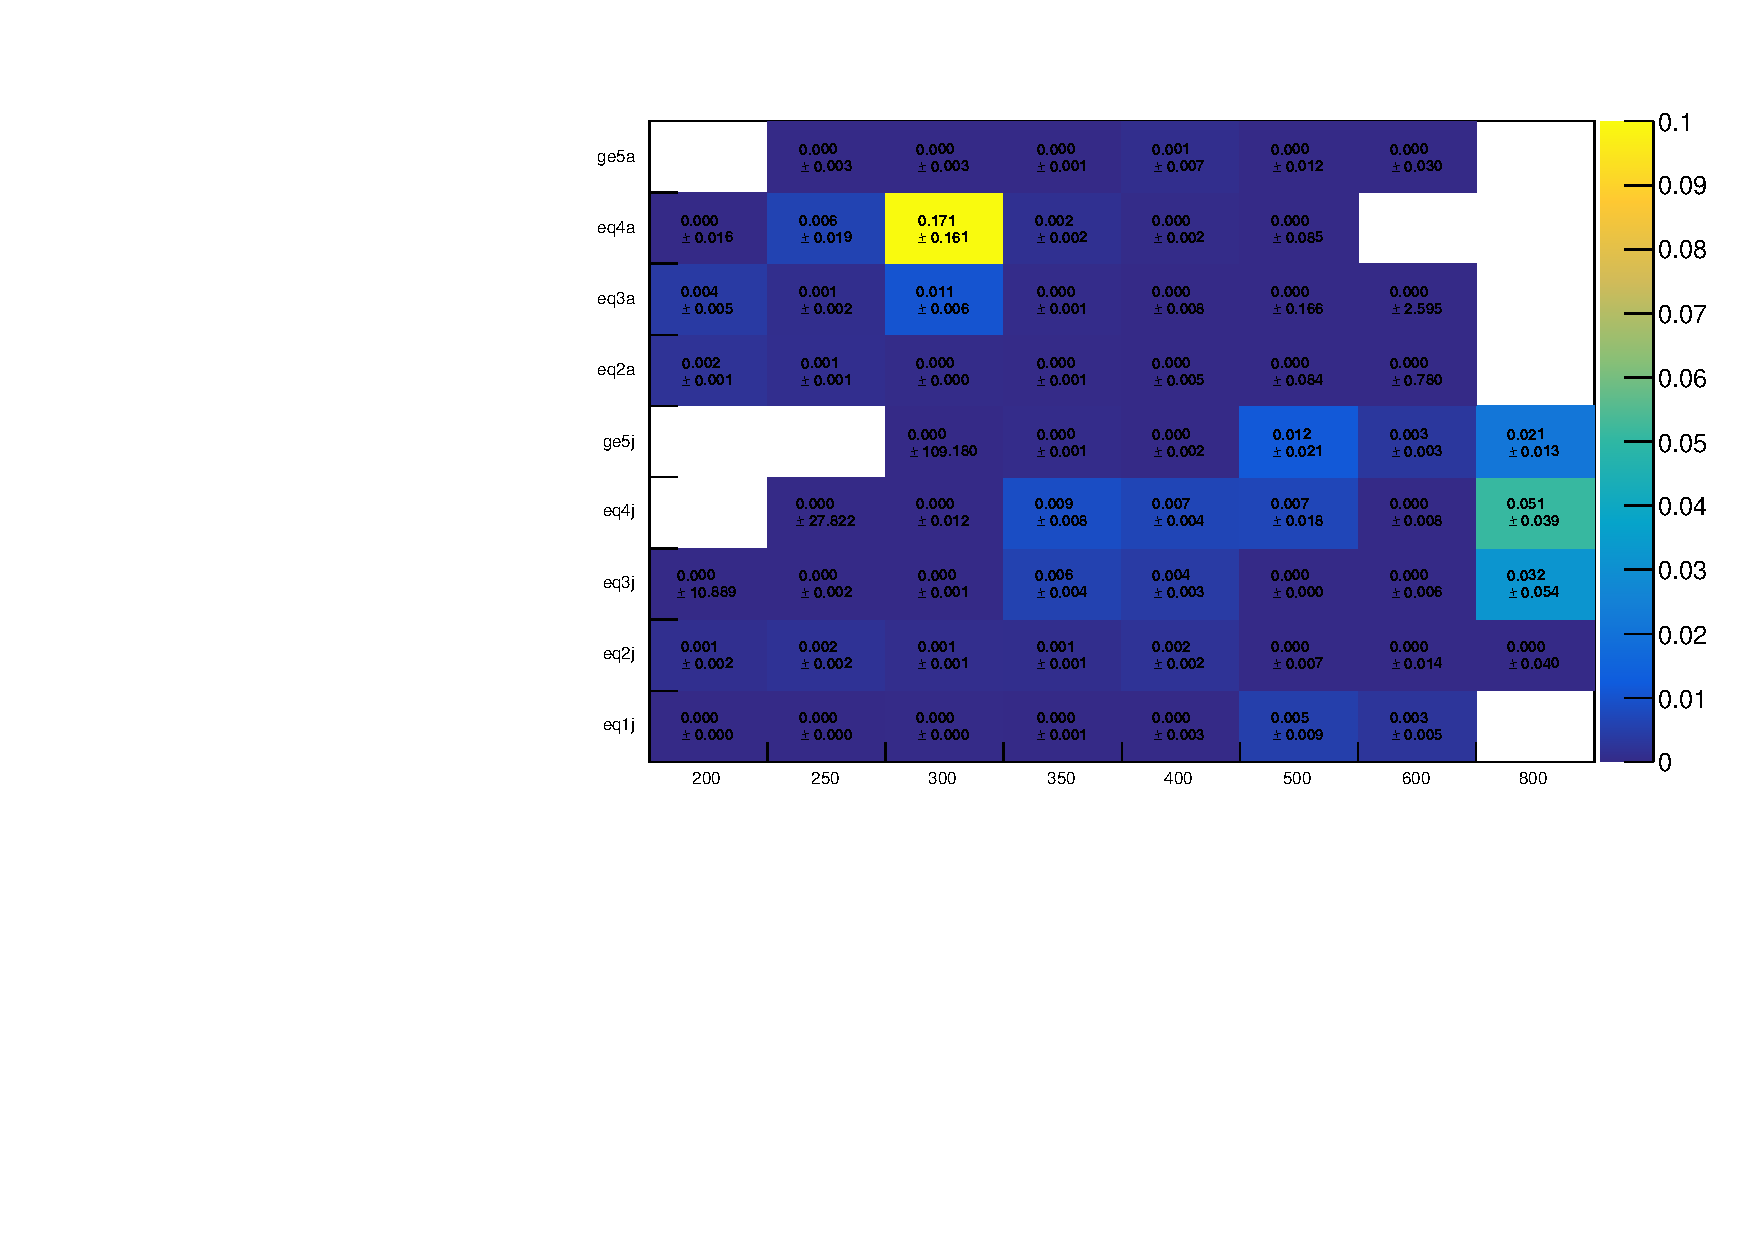
\includegraphics[width=0.5\textwidth]{figures/qcd/plots/predictedQcdDivEwk_Signal}
  } \\
  \caption{The number of events observed in the $\mhtmet>1.25$ sideband, 
    binned according to \njet and \scalht are shown in (a). In
    (b) these yields are corrected by subtracting the expected
    electroweak component. Shown in
    (c) is the result of multiplying the observed multijet events predicted
    in (b) by the translation factor from the sideband to the signal
    region determined with simulation (shown in
    Fig.~\ref{fig:qcd_plots}). This gives a data driven expectation of
    the quantity of multijet background events in the signal region. 
    Finally, (d), shows the ratio of expected
    multijet background events in the signal region divided by
    non-multijet backgrounds. The multijet background is therefore
    shown to be at the percent level.}
  \label{fig:qcd_plots2}
\end{figure}

% THIS IS NOW UNNECESSARY:  
% The data counts in the \mhtmet sideband are collected with the
% \verb!HLT_HTxxx_AlphaT0pyy!  and \verb!HLT_HT800! signal triggers
% described in Sec.~\ref{sec:triggers}. Events satisfy the full signal
% region requirements plus the inverted \mhtmet requirement and are
% binned according to \njet and \scalht. 
% Any contribution from
% non-multijet backgrounds (V+jets, \ttbar, \etc) in each bin is
% estimated from simulation\footnote{In the future, the counts from
%   non-multijet backgrounds will be estimated from the muon data
%   control samples and transfer factors determined from simulation
%   (using the method described in Sec.~\ref{sec:backgroundmet}).} and
% subtracted from the data counts. Any remaining counts, $\mathcal{Q}$,
% are assumed to arise from multijet production.
Figure~\ref{fig:data_fail} shows the observed counts in the \mhtmet
sideband, and Fig.~\ref{fig:data_corr} shows the QCD counts 
in the sideband predicted by the maximum likelihood fit.
Figure~\ref{fig:qcd_pred} shows the predicted counts for the multijet
contribution in the signal region bins, which are obtained from the
products of \rmhtmet and $\mathcal{Q}$, summarised in
Figs.~\ref{fig:qcd_ratio} and \ref{fig:data_corr}. Finally,
Fig.~\ref{fig:qcd_ewk_ratio} shows the ratios of predicted multijet
counts with respect to the expected EWK counts in the signal region.
This allows the quantification of
the (predicted) relative contamination from multijet events in the
signal region bins. The EWK \mht and \nb shapes derived from
simulation are used to predict the distribution 
of QCD events, this approach is validated in
Sec.~\ref{sec:qcdValidation}. 

%% The predictions summarised in Fig.~\ref{fig:qcd_ewk_ratio} support the
%% expectation based on experience with 8~TeV data that the \HT-dependent
%% \alphat thresholds defined in Table~\ref{tab:sr-selections} and the
%% requirement of $\bdphi > 0.5$ are sufficient to reduce the multijet
%% contamination in all bins of the signal region to the sub-percent with
%% respect to the total non-multijet background. With this level of
%% suppression, it is expected that the uncertainty associated with the
%% residual multijet contamination to be sub-dominant with respect to,
%% and fully absorbed by, the systematic uncertainties on the non-multijet
%% backgrounds, which are expected to be at the level of $\sim$10\% or
%% larger. 

The predictions summarised in Fig.~\ref{fig:qcd_ewk_ratio} show that 
the \HT-dependent \alphat thresholds defined in Table~\ref{tab:sr-selections} 
and the requirement of $\bdphi > 0.5$ suppress the multijet
contamination in all bins of the signal region to percent-level or smaller with
respect to the total non-multijet background. These predicted multijet events are 
included as a background contribution to the likelihood model
described in Sec~\ref{sec:likelihood}.


\subsection{Validation of the QCD prediction}
\label{sec:qcdValidation}

Despite being as data driven as possible, the method for predicting the QCD contamination in the signal region
described in Sec.~\ref{sec:qcdMethod} relies on the ratio, \rmhtmet,
of QCD counts
that is derived with simulation. This ratio is validated with data in a
QCD enriched sideband, where full signal region selection is used
other than
an inversion of the \bdphi cut to $\bdphi<0.5$. In this sideband a
data driven estimation of the QCD counts is carried out in two regions, those with \mhtmet values less than
1.25 and those with values greater than 1.25. These predictions are
made with a maximum likelihood
fit, analagous to that described in Sec.~\ref{sec:qcdMethod}. This fit
estimates the EWK counts with single muon, double muon and single
photon control regions and all relevant systematic errors. The
remaining data counts are then attributed to QCD. With this estimation 
of QCD it is possible to derive a data driven ratio of QCD counts with 
$\mhtmet<1.25$ and those with $\mhtmet>1.25$, $\rmhtmet_{\bdphi<0.5}^{data}$. By
taking MC counts in the \bdphi sideband it is also possible to
calculate the \mhtmet simulation ratio, $\rmhtmet_{\bdphi<0.5}$. 

To
validate the ratio \rmhtmet it is assumed that if the simulation of
the ratio in the \bdphi sideband agrees with that
derived from data, the simulated ratio that is not in the sideband
is valid. Any disagreement is covered by 
a systematic error on the signal region QCD prediction. The double ratio of
$\rmhtmet_{\bdphi<0.5}$ and $\rmhtmet_{\bdphi<0.5}^{data}$ in \scalht
and \njet bins is shown in Fig.~\ref{fig:RR_qcd}. Bins in which there
are insufficient statistics in data or simulation to make the calculation are left out.
This
plot illustrates that a fully correlated systematic of 100\% taken on the
predicted QCD contamination in the signal region should cover any
disagreement between simulation and data.

\begin{figure}[h!]
  \begin{center}        
    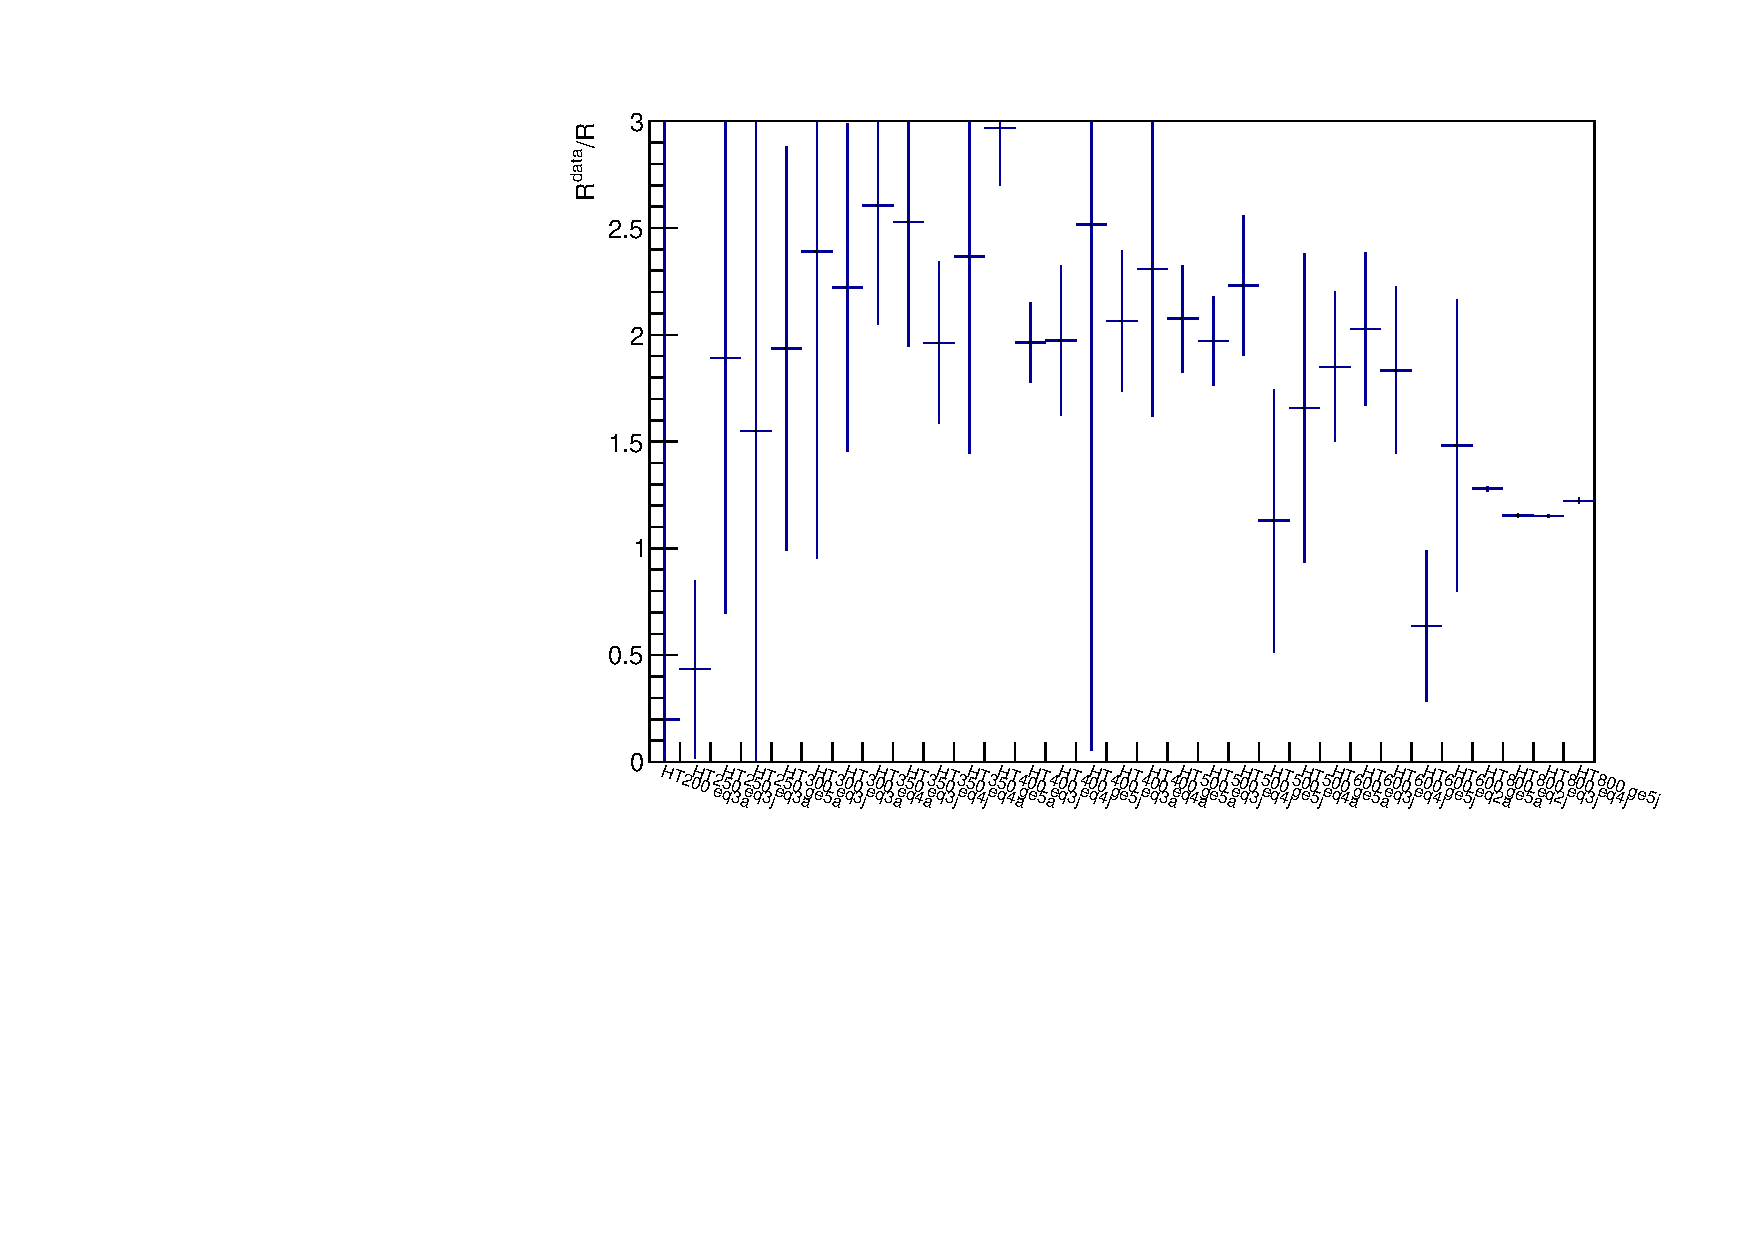
\includegraphics[width=\textwidth]{figures/qcd/plots/doubleQcdSbSrRatio1D}
    \caption{ Ratio of the measurement of \rmhtmet, the pass/fail ratio for the \mhtmet selection, from data and Monte Carlo in the $\bdphi < 0.5$ sideband in (\scalht, \njet) bins.  
    }

    \label{fig:RR_qcd}
  \end{center} 
\end{figure}

As the prediction of QCD in the signal region is carried out
inclusively over \nb and \mht, the QCD shapes for these variables are
taken from the EWK simulation and normalised to the QCD counts. 
A lack of statistics in
the QCD MC led to the adoption of this approach. To validate it, the simulated \mht distributions
for the QCD and EWK processes in the signal region are divided. This is shown in
Figs.~\ref{fig:asym_qcd_validation}-\ref{fig:asym_qcd_validation}.
As the normalisation is carried out independently, a flat distribution
of the ratio is enough for validation. Within uncertainties, the level of agreement is acceptable given the
small total QCD contribution to the signal region and its large
systematic uncertainty. 

\begin{figure}[h!]
  \begin{center}
    \subfigure[{ Asymmetric,
    $\scalht<400$~GeV}]{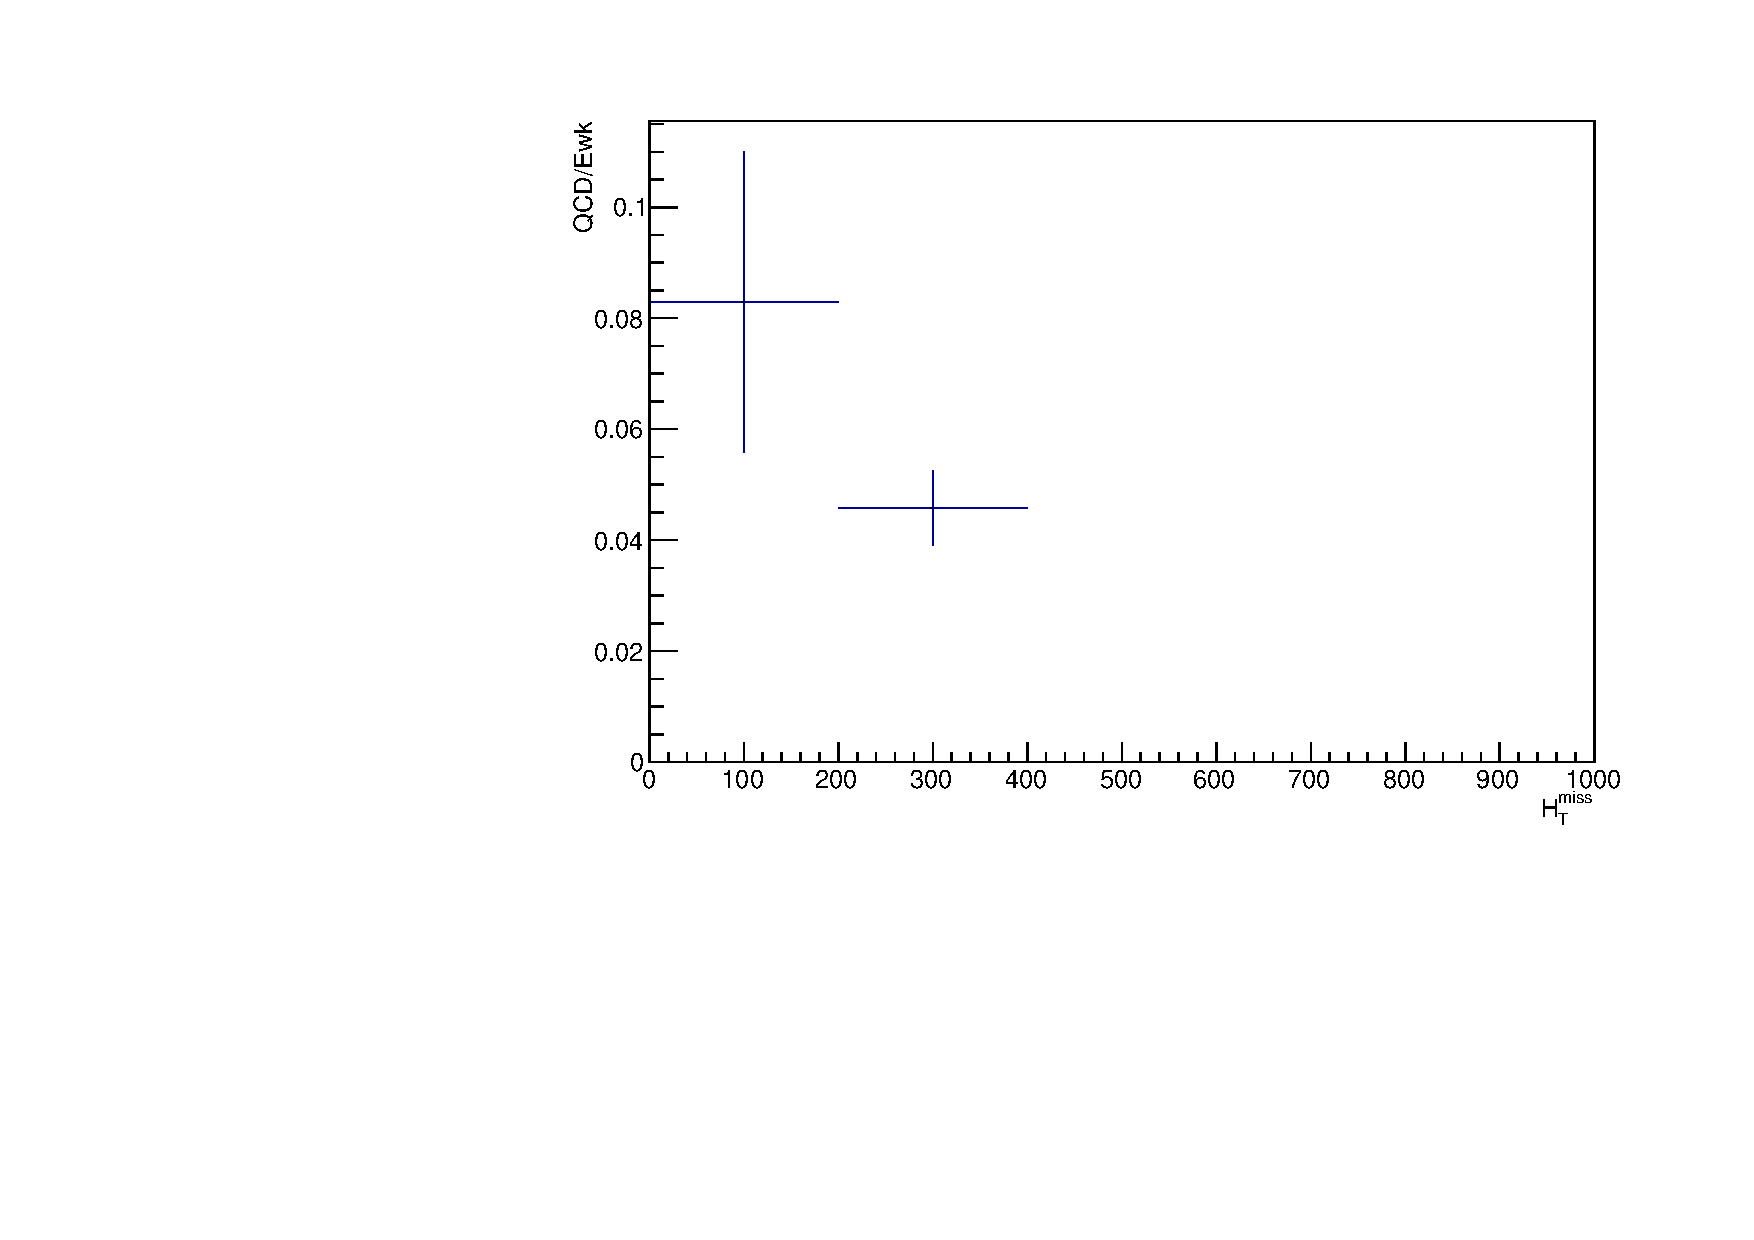
\includegraphics[width=0.5\textwidth]{figures/qcd/plots/mht_ht_lt400asym}} ~~
    \subfigure[{ Asymmetric,
    $\scalht<400$~GeV}]{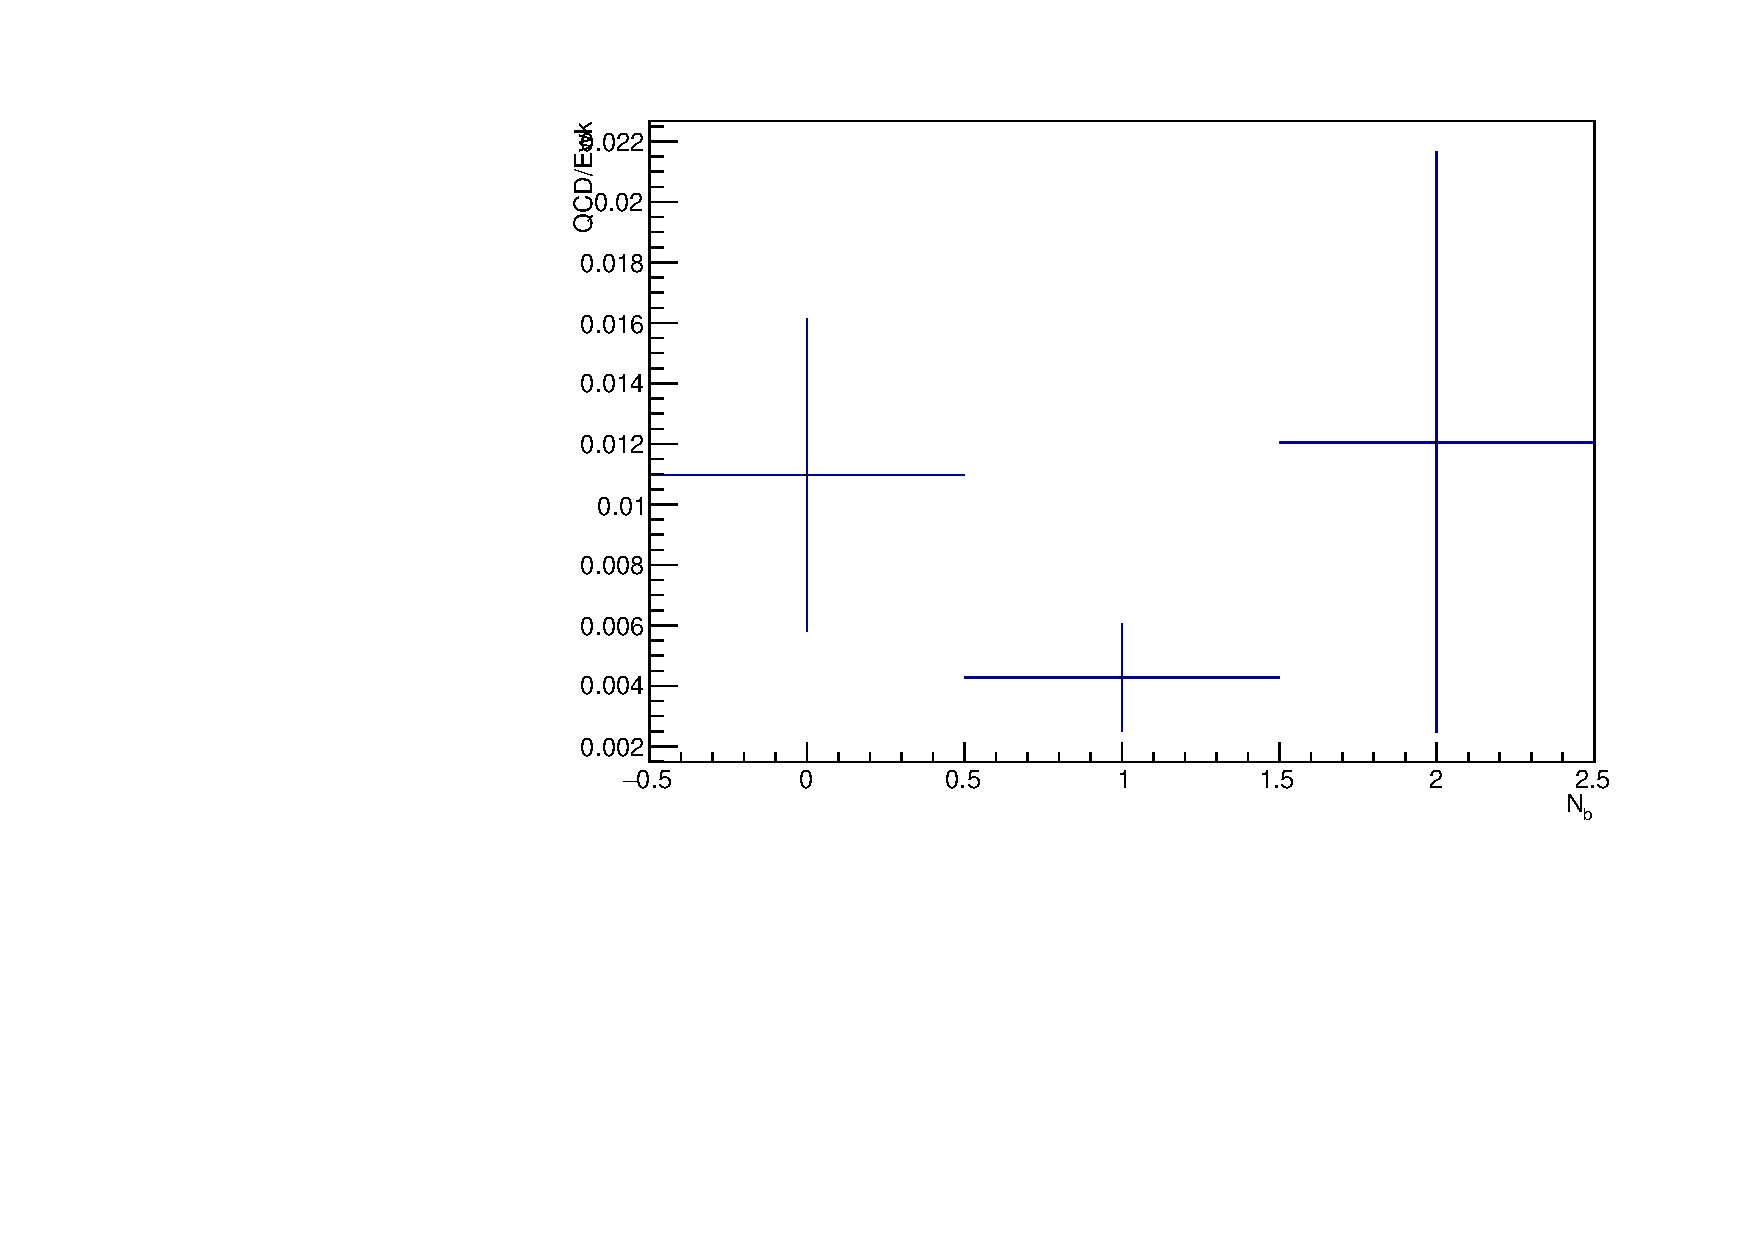
\includegraphics[width=0.5\textwidth]{figures/qcd/plots/nB_ht_lt400asym}} \\
    \subfigure[{ Asymmetric,
    $400<\scalht<800$~GeV}]{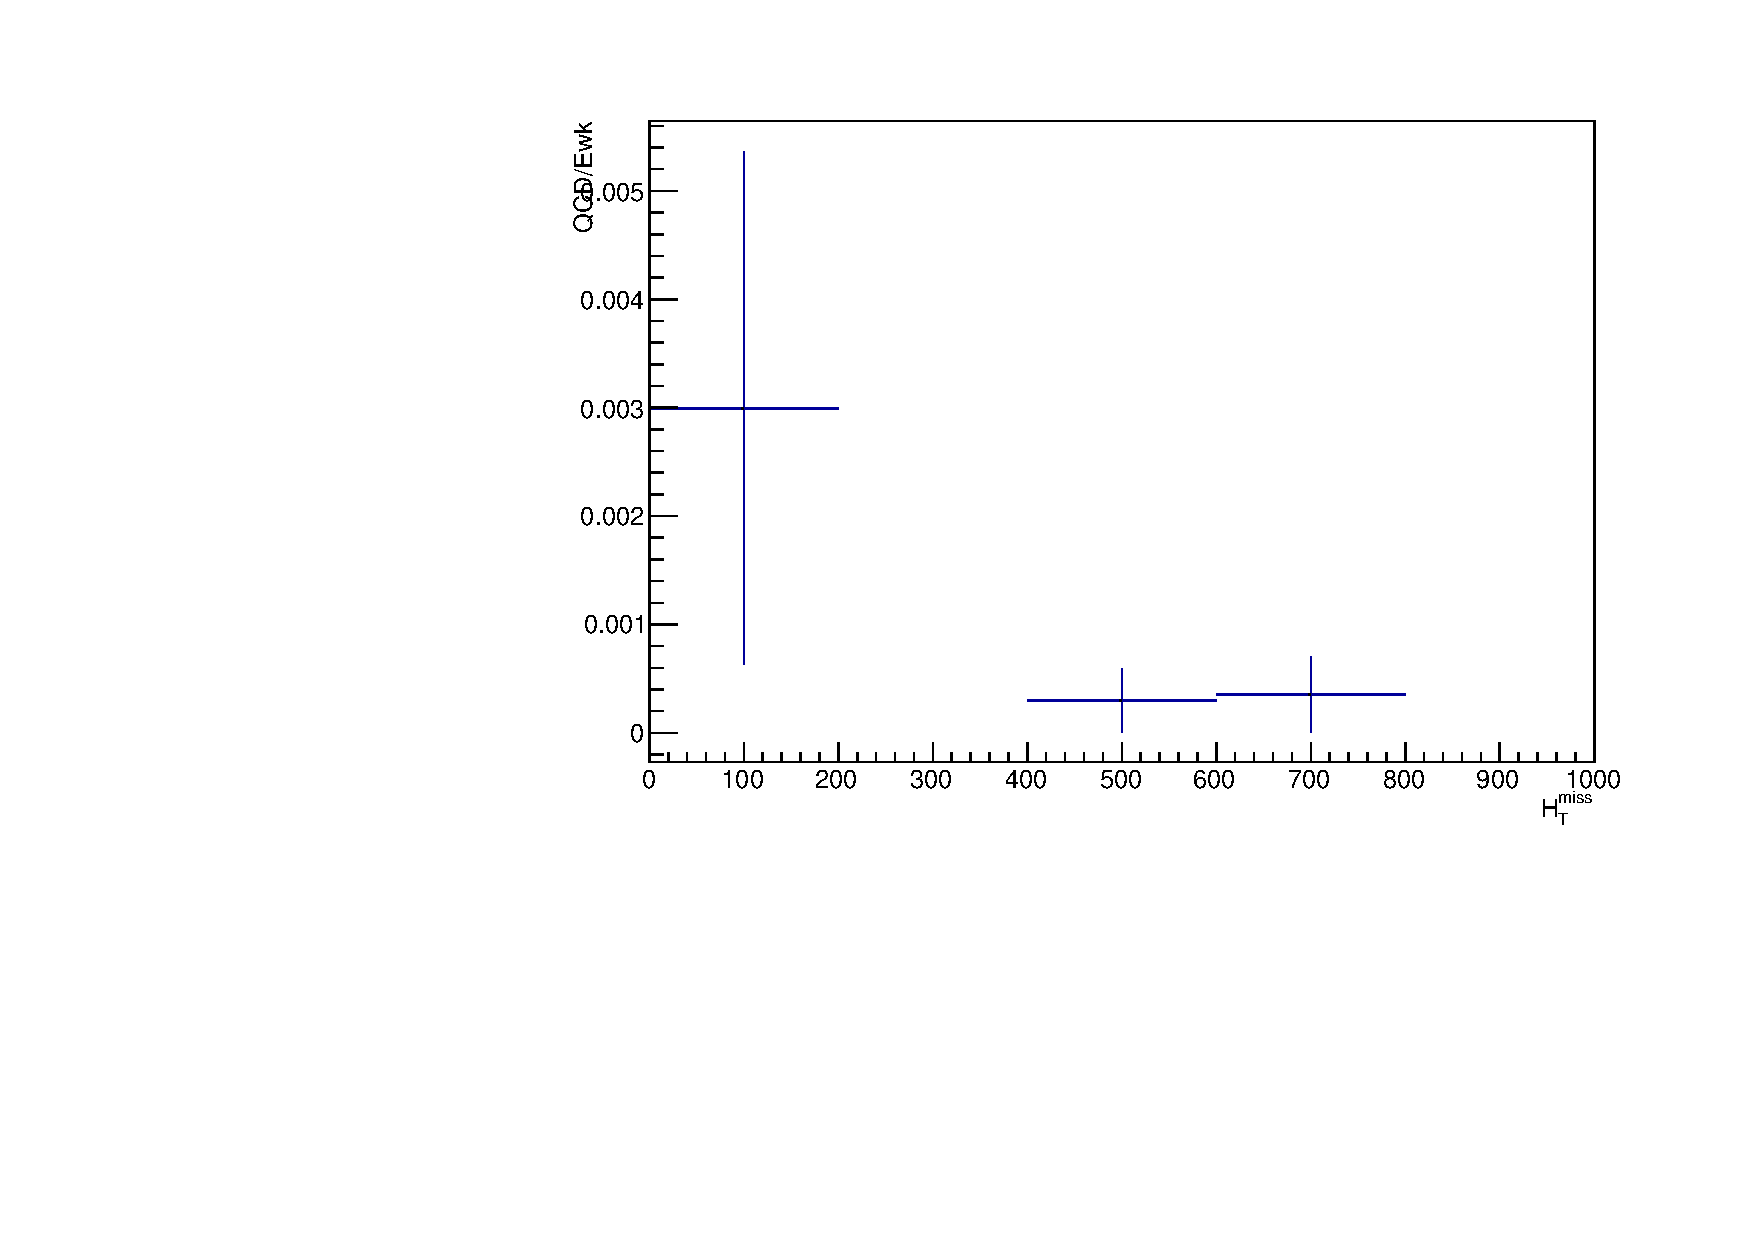
\includegraphics[width=0.5\textwidth]{figures/qcd/plots/mht_ht_lt800asym}} ~~
    \subfigure[{ Asymmetric,
    $400<\scalht<800$~GeV}]{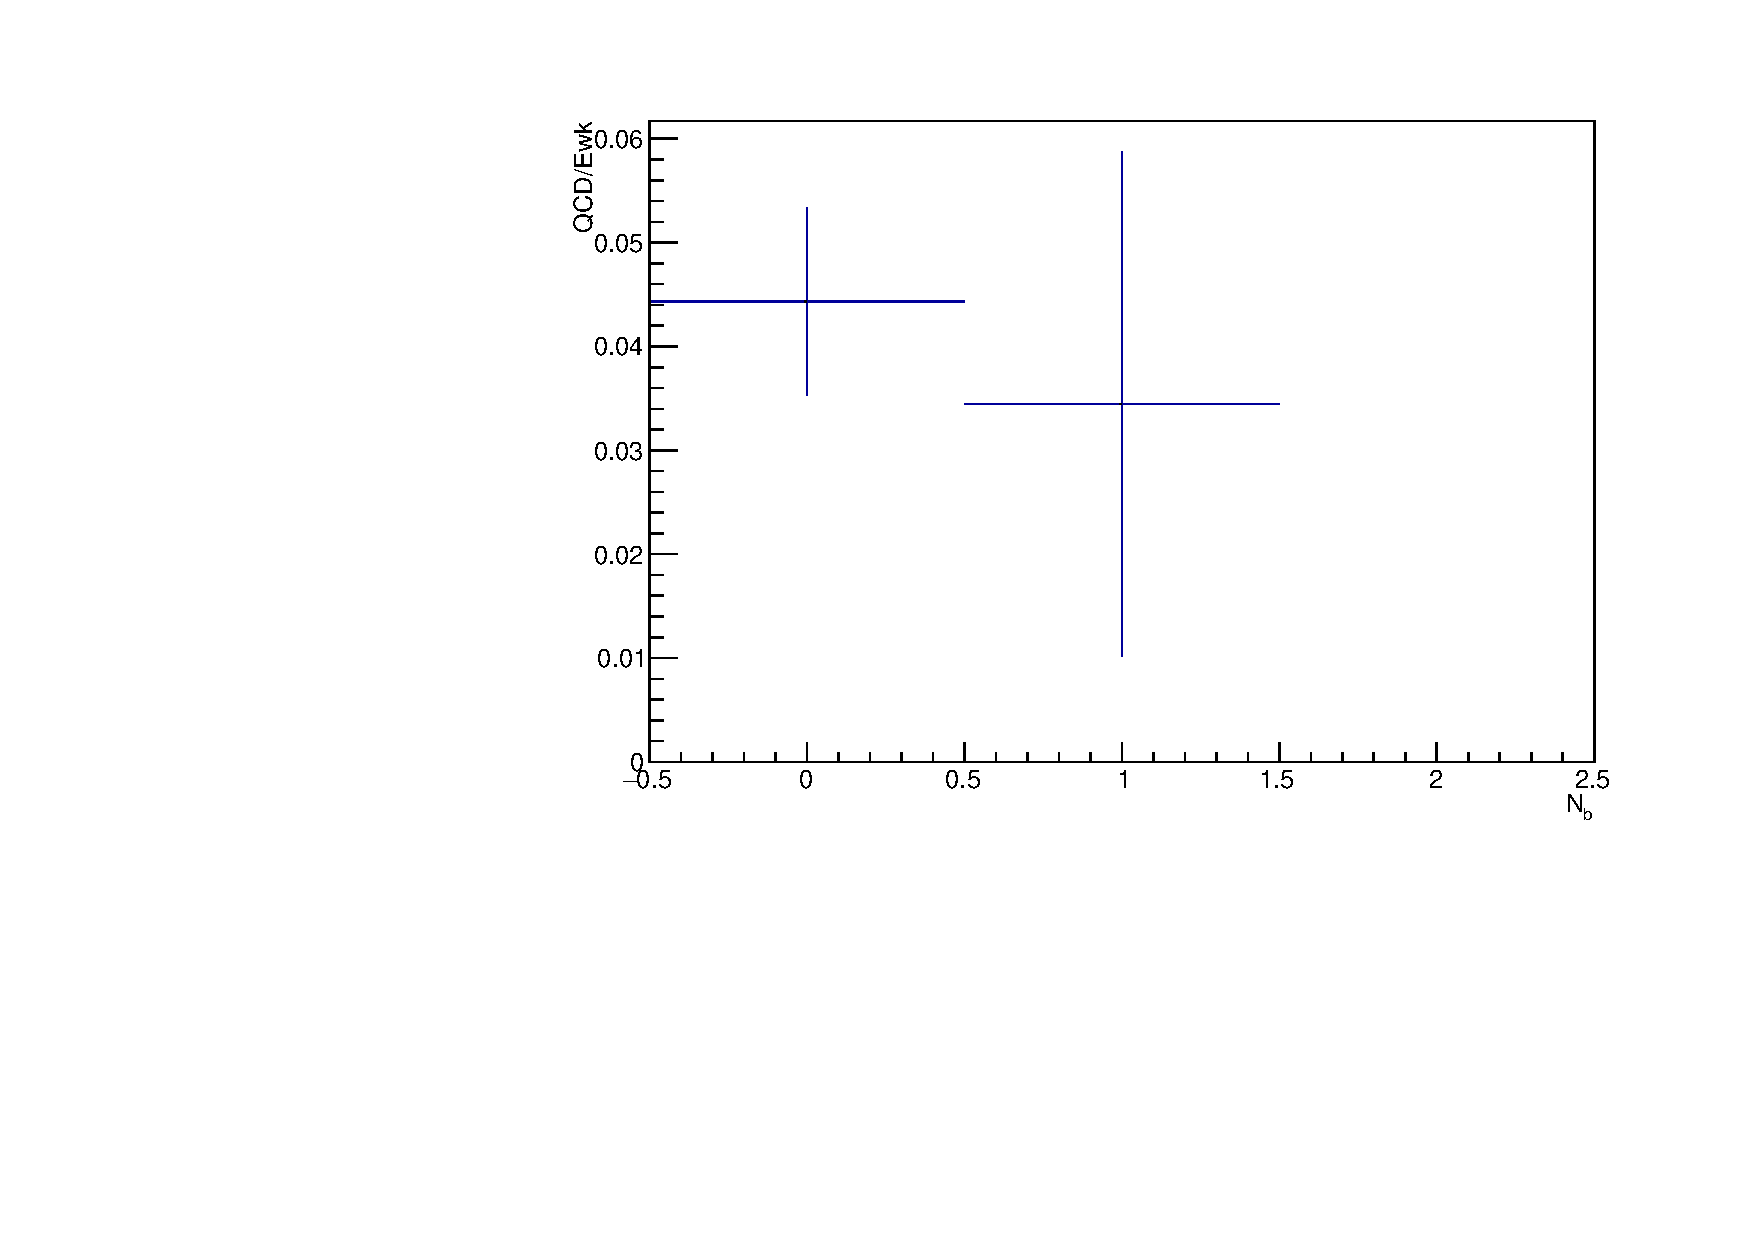
\includegraphics[width=0.5\textwidth]{figures/qcd/plots/nB_ht_lt800asym}} \\
    \caption{ Ratio of QCD to electroweak Monte Carlo prediction in the signal region for different \scalht selections as a function of \mht (Left) and $\nb$ (Right) for the asymmetric jet category. A constant fit to the data is represented by the red line, with the $\pm$100\% uncertainty represented by the blue hashed region.
    }
    \label{fig:asym_qcd_validation}
  \end{center} 
\end{figure}


\clearpage
\begin{figure}[h!]
  \begin{center}
    \subfigure[{ Symmetric,
    $\scalht<400$~GeV}]{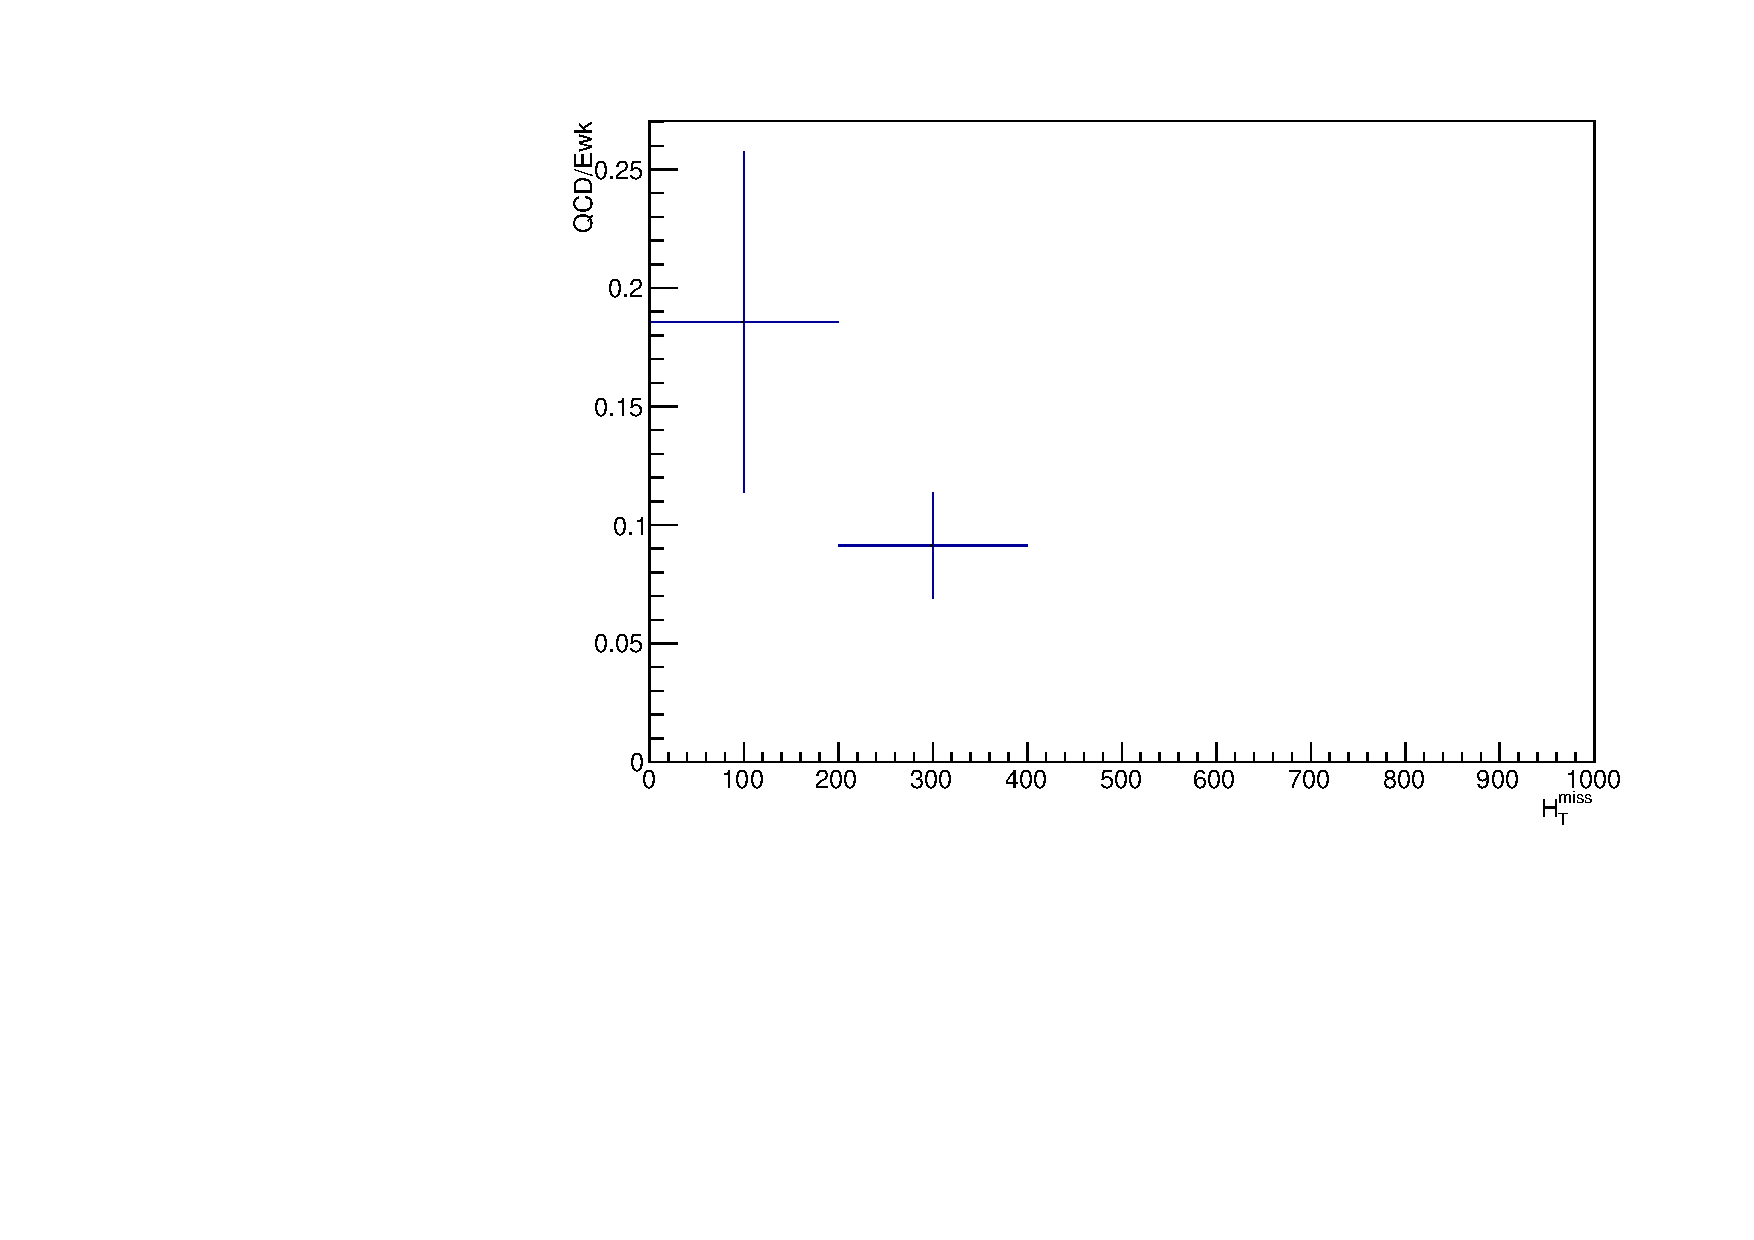
\includegraphics[width=0.5\textwidth]{figures/qcd/plots/mht_ht_lt400sym}} ~~
    \subfigure[{ Symmetric,
    $\scalht<400$~GeV}]{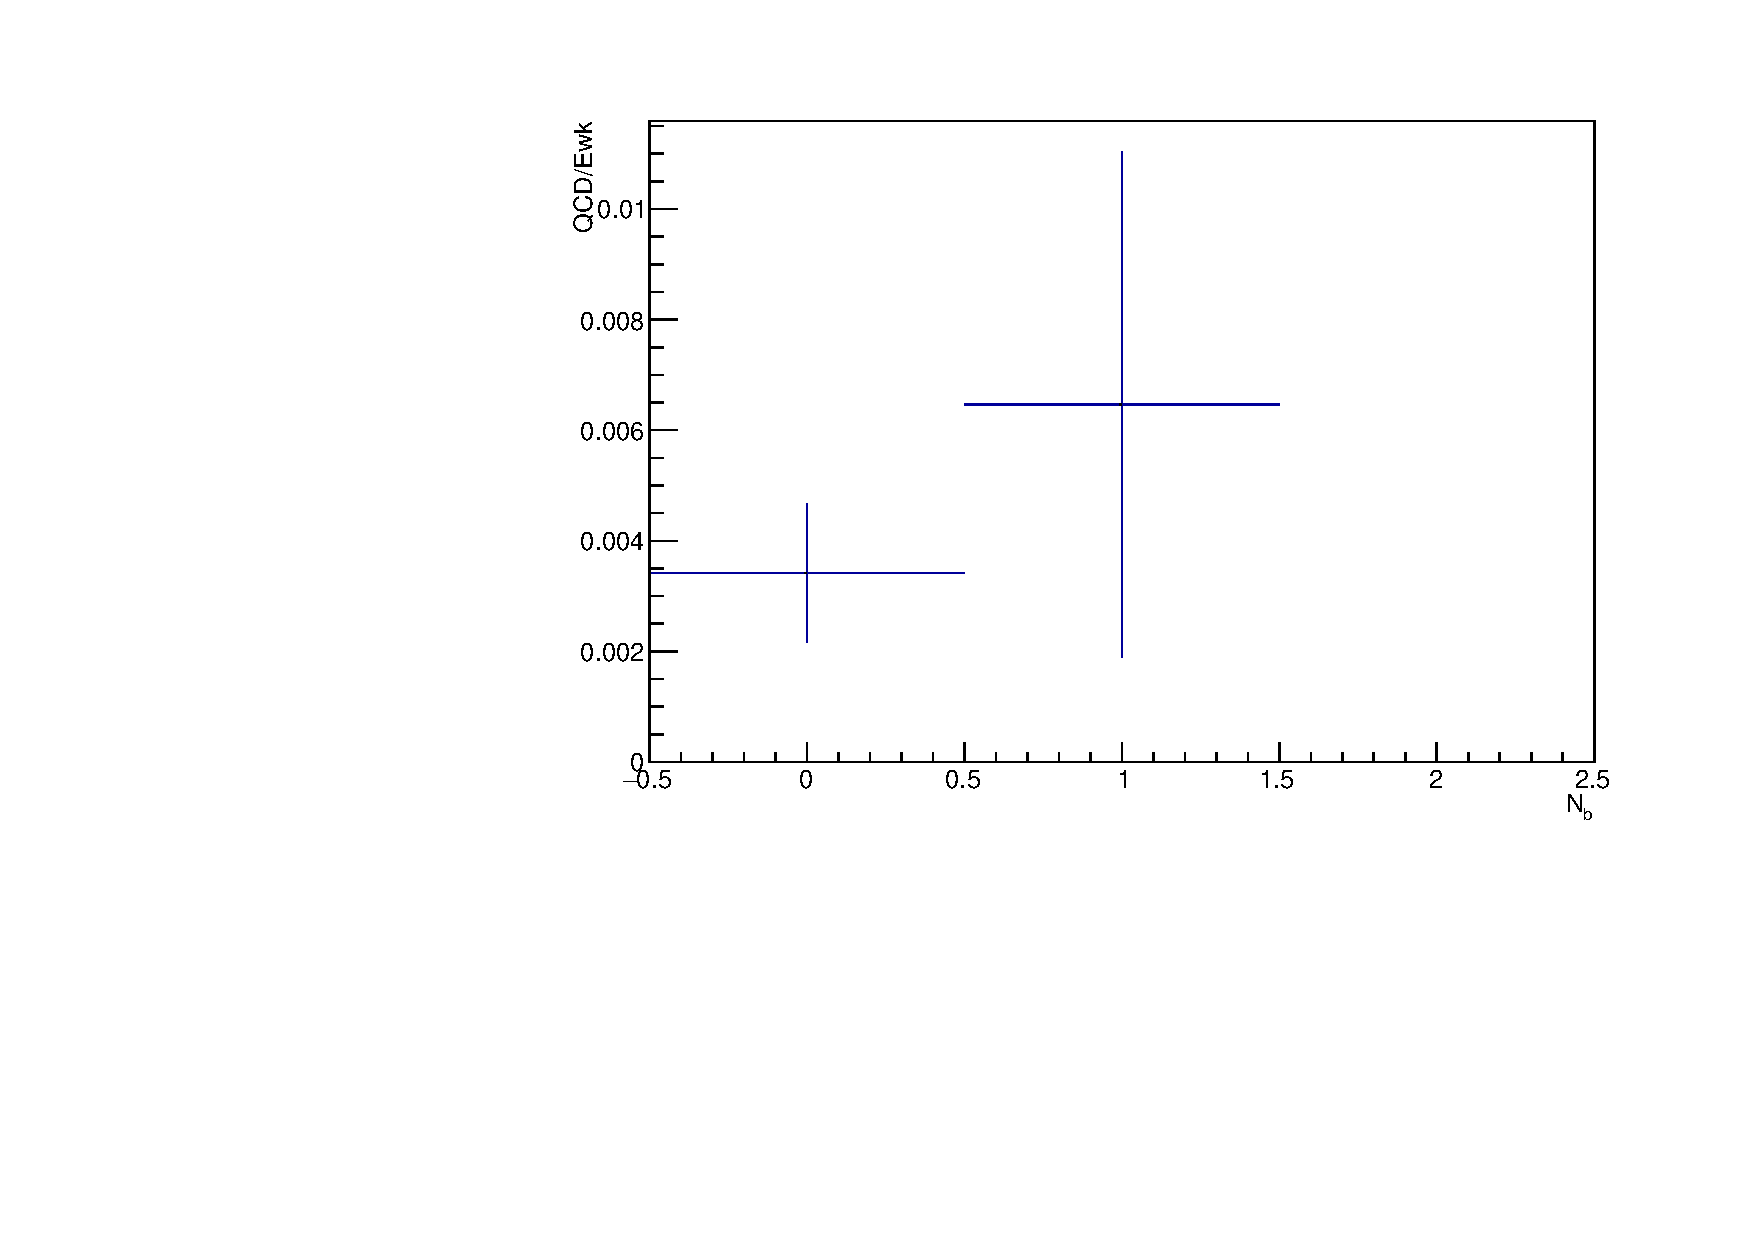
\includegraphics[width=0.5\textwidth]{figures/qcd/plots/nB_ht_lt400sym}} \\
    \subfigure[{ Symmetric,
    $400<\scalht>800$~GeV}]{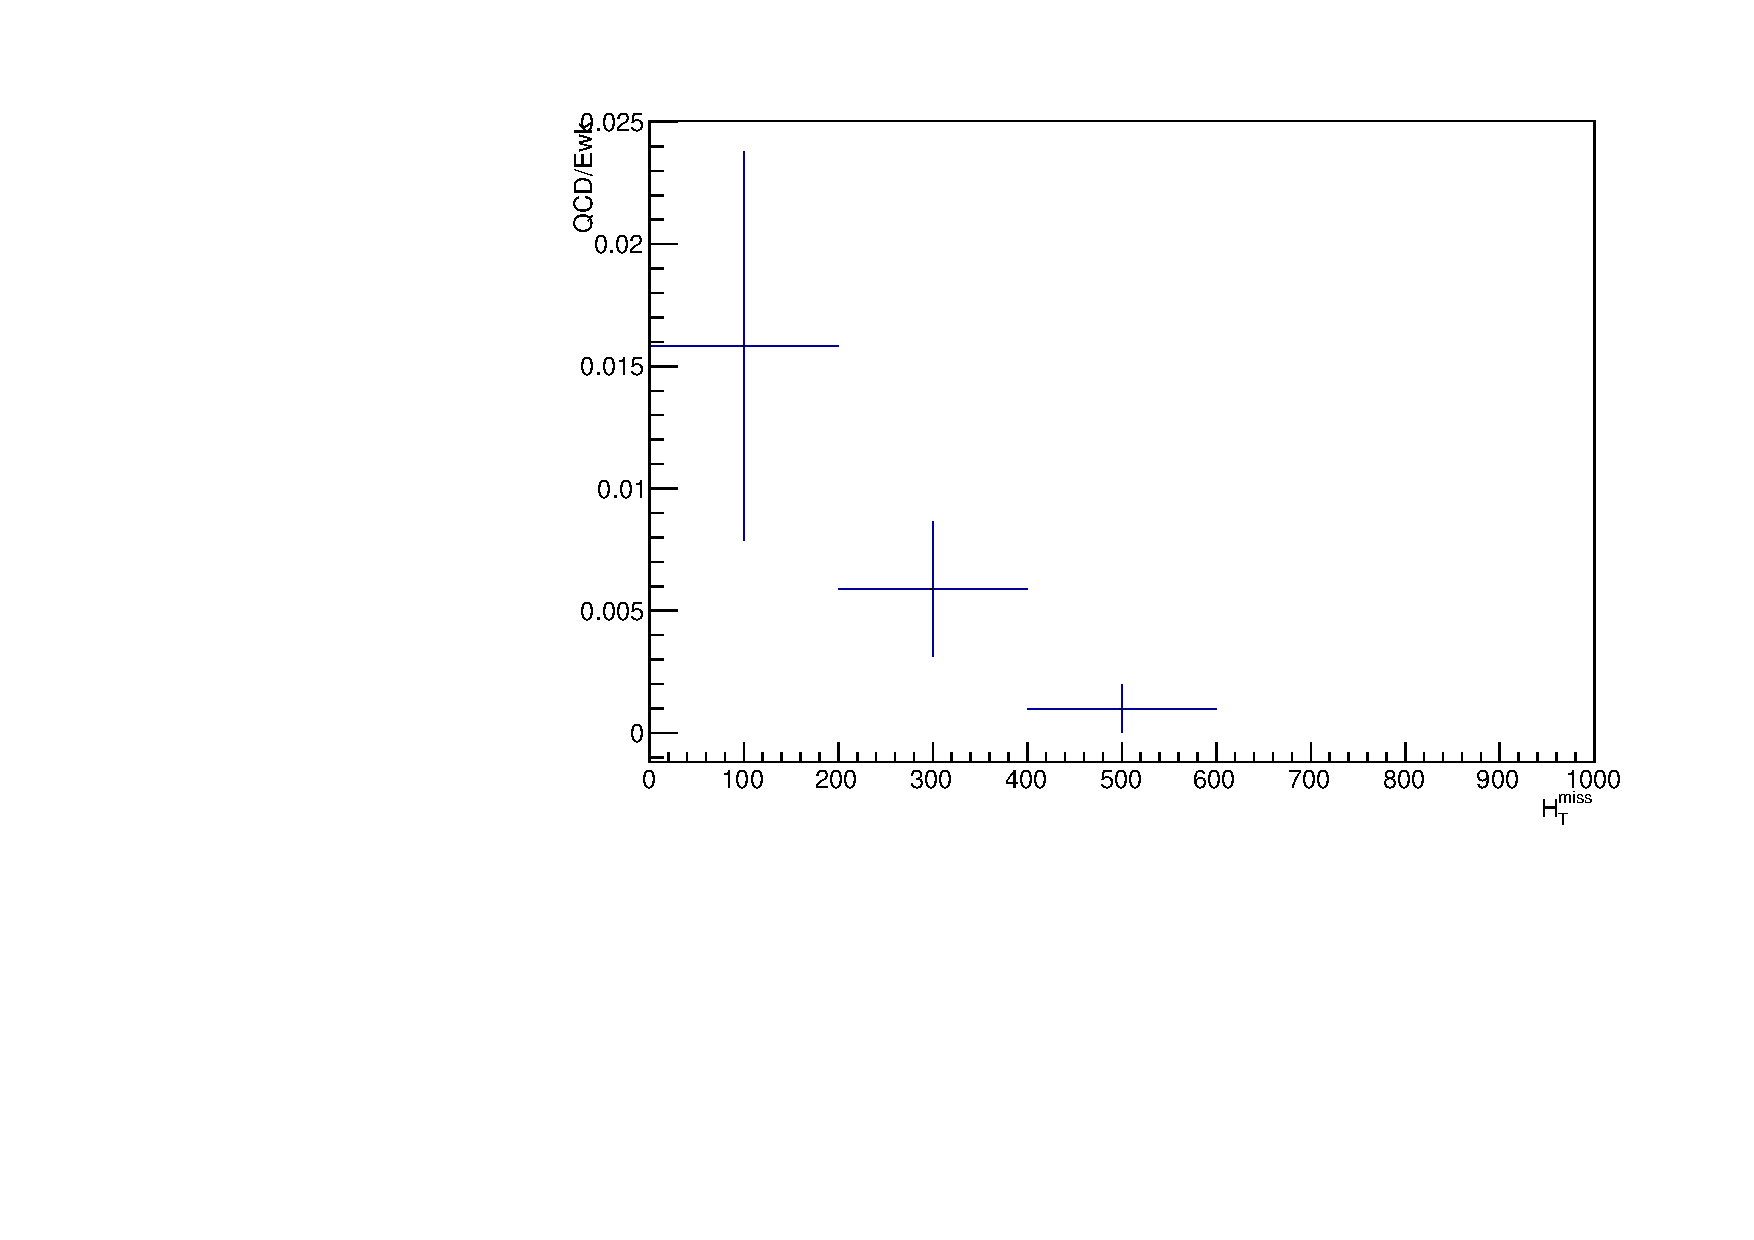
\includegraphics[width=0.5\textwidth]{figures/qcd/plots/mht_ht_lt800sym}} ~~
    \subfigure[{ Symmetric,
    $400<\scalht<800$~GeV}]{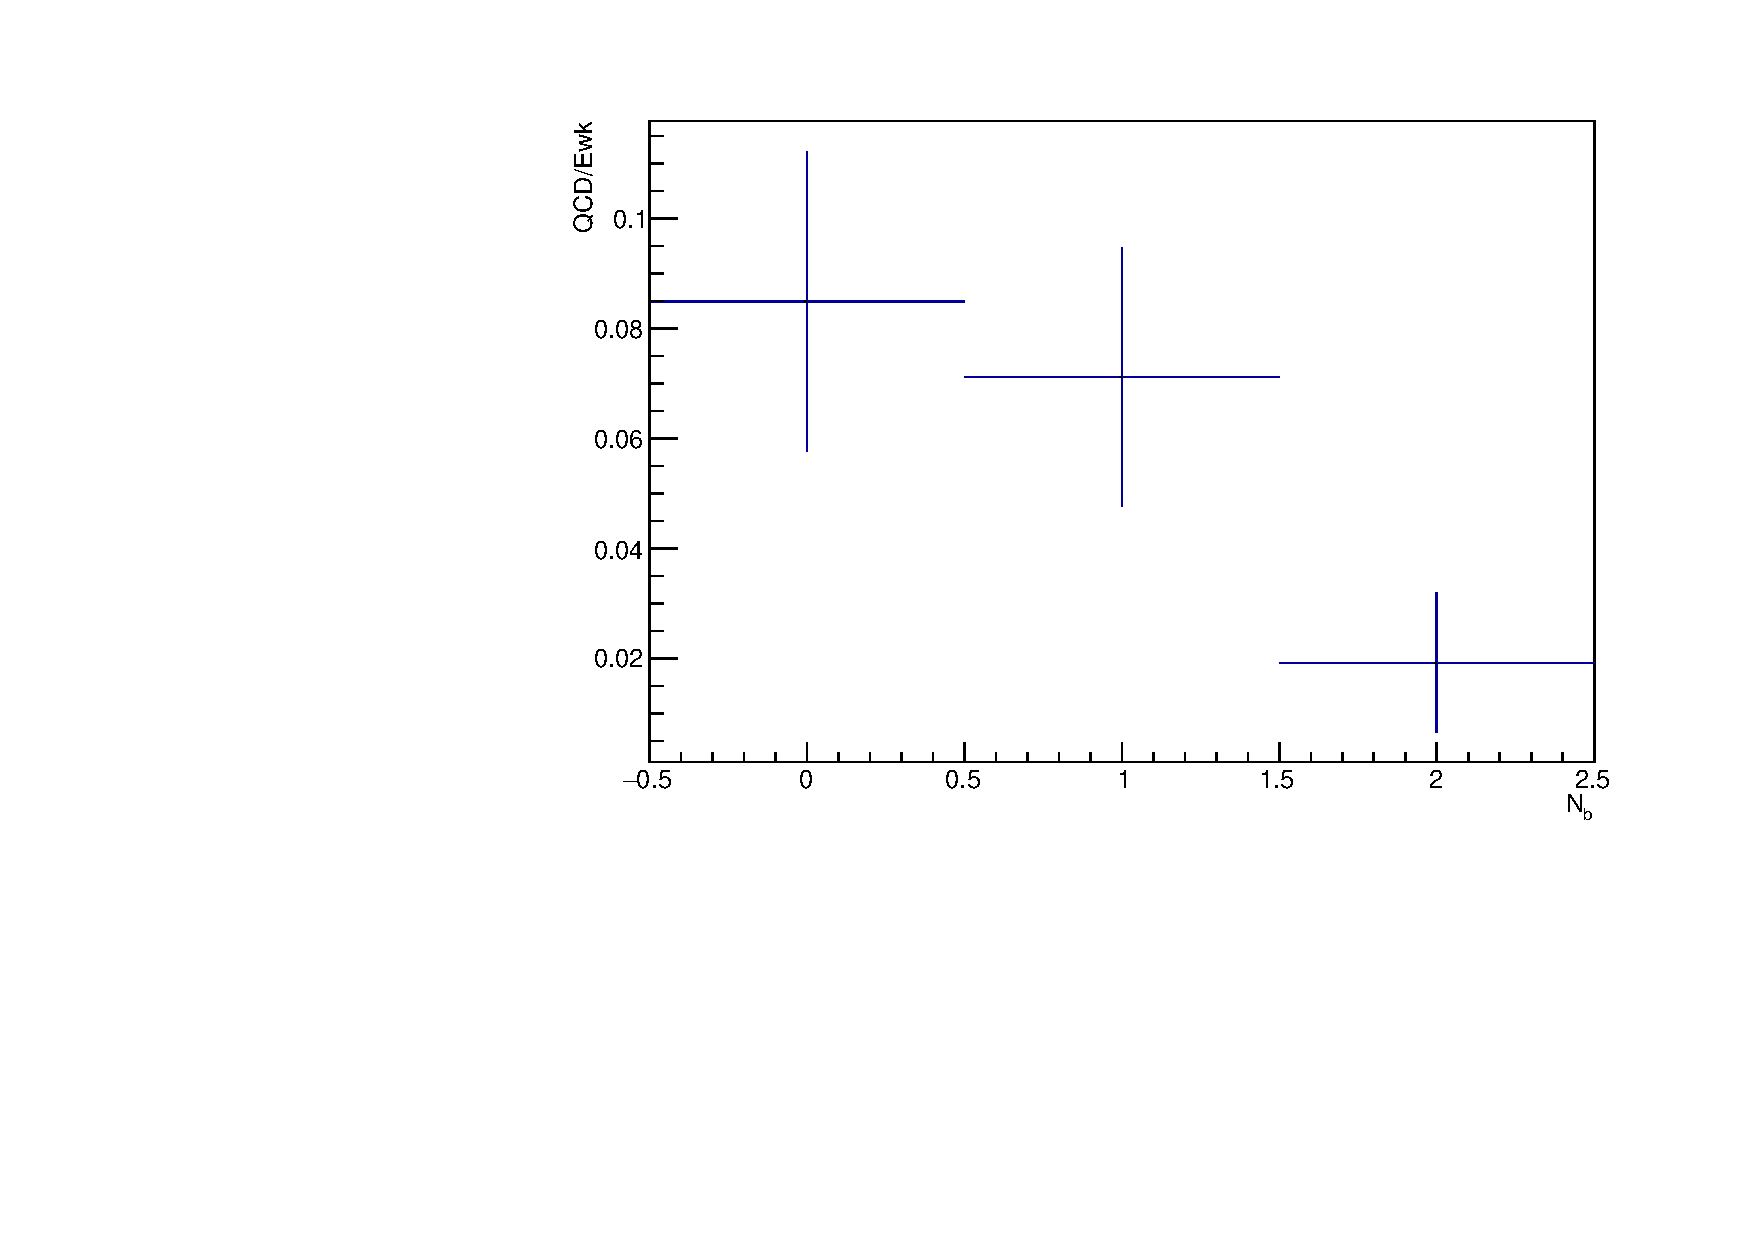
\includegraphics[width=0.5\textwidth]{figures/qcd/plots/nB_ht_lt800sym}} \\
    \subfigure[{ Symmetric,
    $\scalht>800$~GeV}]{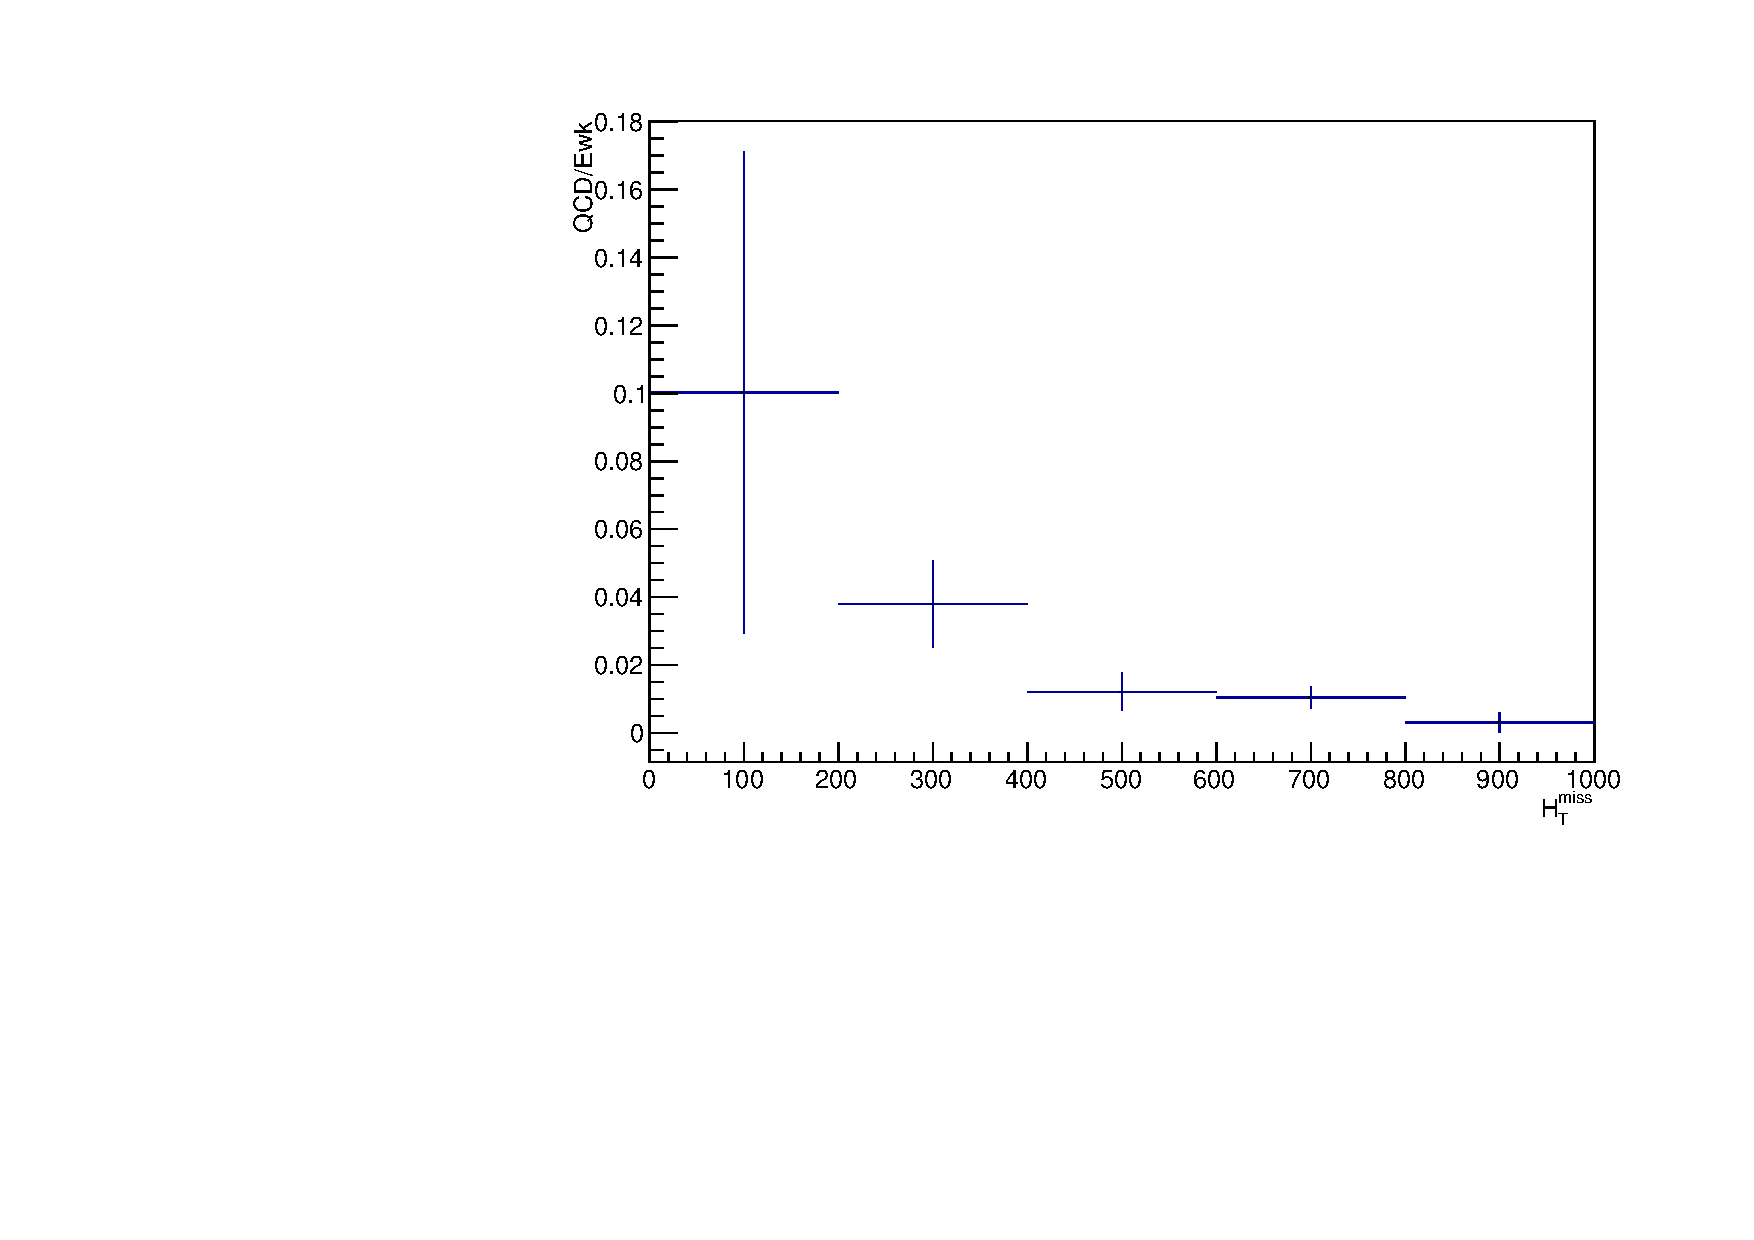
\includegraphics[width=0.5\textwidth]{figures/qcd/plots/mht_ht_ltInfsym}} ~~
    \subfigure[{ Symmetric,
    $\scalht>800$~GeV}]{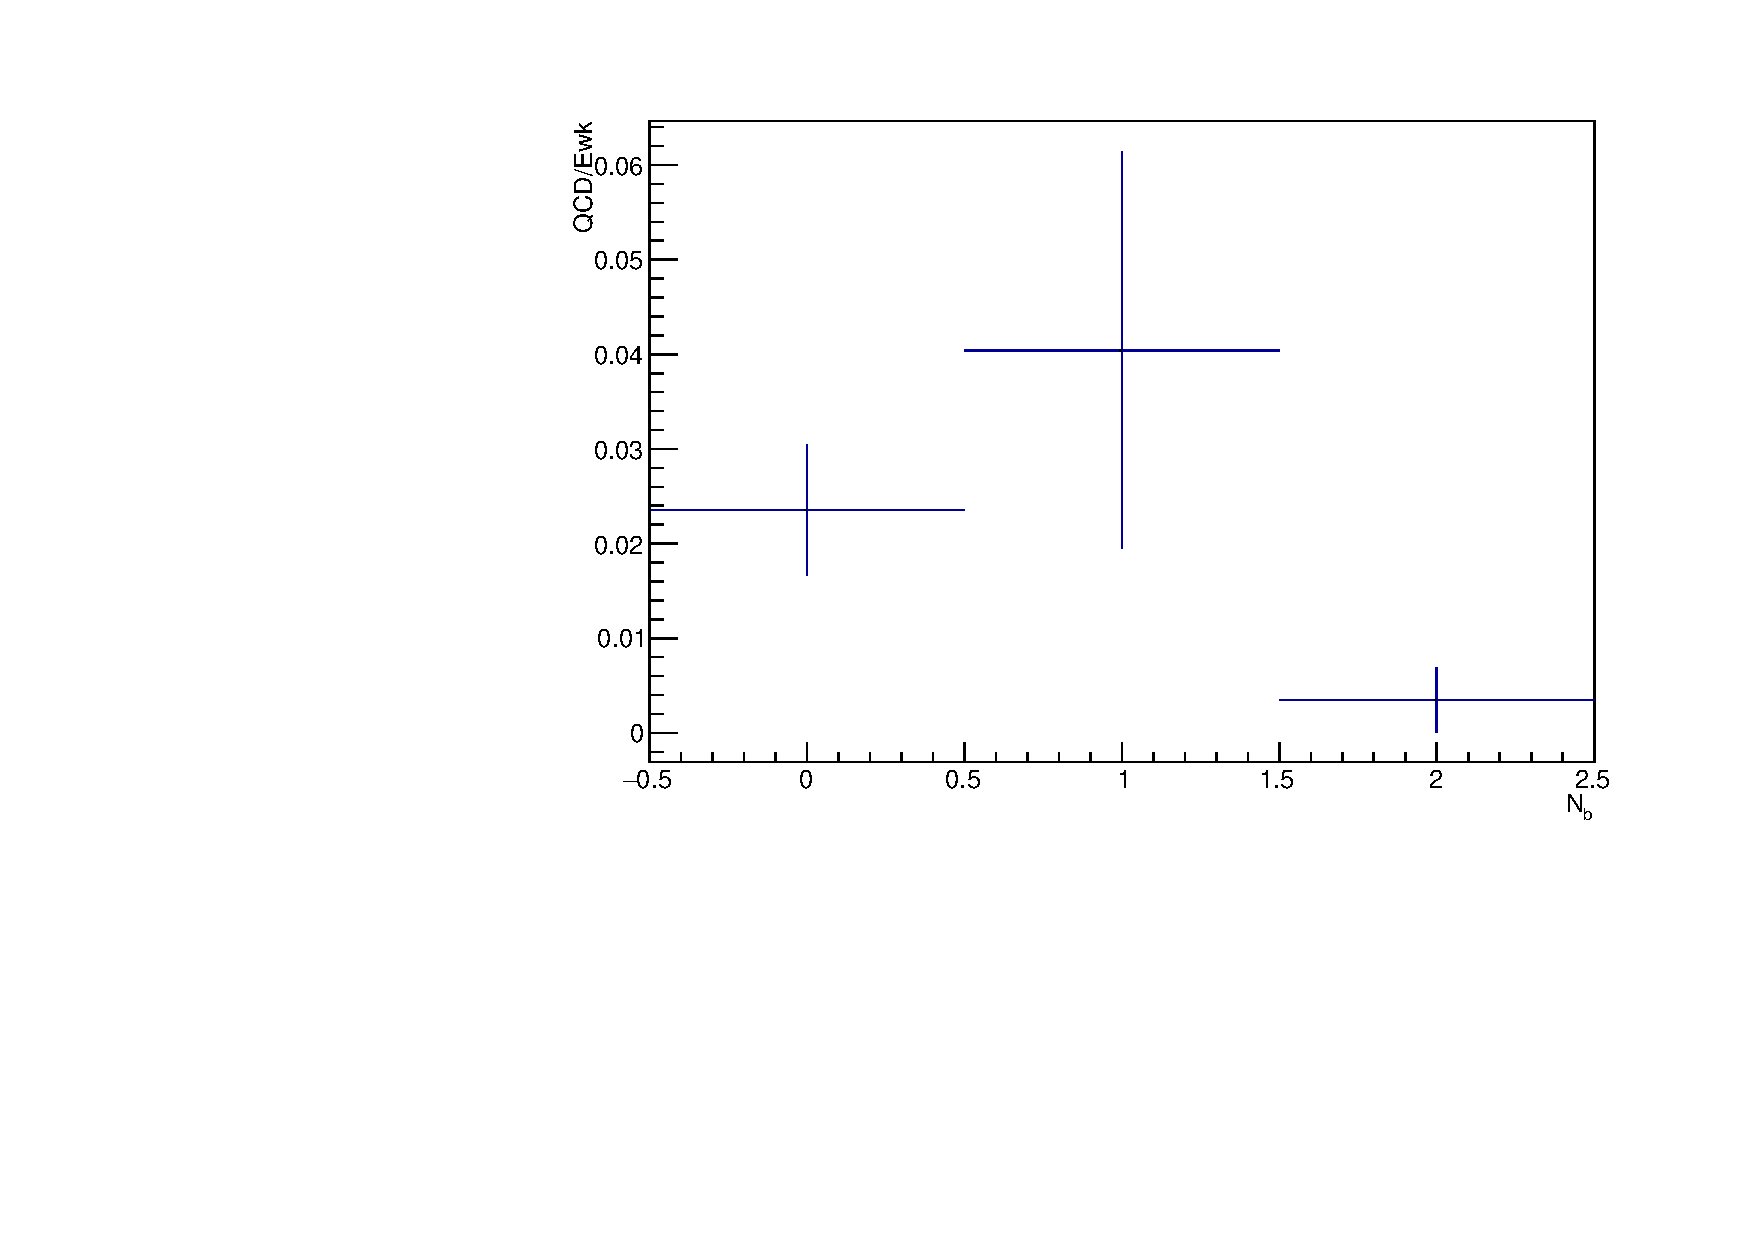
\includegraphics[width=0.5\textwidth]{figures/qcd/plots/nB_ht_ltInfsym}} \\
      \caption{ Ratio of QCD to electroweak Monte Carlo prediction in the signal region for different \scalht selections as a function of \mht (Left) and $\nb$ (Right) for the asymmetric jet category. A constant fit to the data is represented by the red line, with the $\pm$100\% uncertainty represented by the blue hashed region.
    }
    \label{fig:sym_qcd_validation}
  \end{center} 
\end{figure}
